\documentclass[8pt]{extarticle}
\usepackage[top=0in, bottom=0in, left=0.1in, right=0.1in]{geometry} % Adjust margins individually
\usepackage{amsmath,amssymb,amsthm}
\usepackage{enumitem}
\usepackage{graphicx} % Required for \includegraphics
\usepackage{ragged2e}

\usepackage[absolute,overlay]{textpos}
\usepackage{array} % For better column definitions
\usepackage{booktabs} % For improved table aesthetics
\raggedbottom
\setlist[itemize]{leftmargin=2em}
\newcommand{\dist}[2]{\left\langle #1,\, #2 \right\rangle}
\setlength{\TPHorizModule}{0.1mm} % Set horizontal units to millimeters
\setlength{\TPVertModule}{0.1mm}  % Set vertical units to millimeters
\usepackage{multicol}
\setlength{\leftmargini}{1.1em} % Adjust the left margin (default is 1.5em)
\setlength{\parskip}{5pt plus 1pt minus 1pt}
\usepackage{setspace}
\setstretch{1}
\pagestyle{empty}

% Redefine the textblock environment
\let\originaltextblock\textblock
\let\endoriginaltextblock\endtextblock

\renewenvironment{textblock}[2][]{%
    \originaltextblock[#1]{#2}%
    \fcolorbox{red}{white}{%
    \begin{minipage}{#2}%
}{%
    \end{minipage}%
    }%
    \endoriginaltextblock
}

\setlist[itemize]{leftmargin=1.2em}
\begin{document}
\begin{titlepage}
    \centering
    \vspace*{1cm}
    {\fontsize{30}{36}\selectfont \textbf{Computer Systems - CheatSheet}} \\
    \vspace{10px}
    {\fontsize{15}{30}\selectfont IN~BA4 - Katerina Argyraki} \\
    \vspace*{10px}
    {\fontsize{15}{20}\selectfont Notes by Ali EL AZDI} \\
    \vfill

    \begin{justify}
        \textit{\large A Computer Systems Cheatsheet has been authorized for the upcoming exam, and I'm sharing a copy of mine for anyone interested. It provides a concise summary of the key concepts and techniques covered in the course. For any updates or suggestions, feel free to reach out to me on Telegram at \texttt{elazdi\_al} or via EPFL email at \texttt{ali.elazdi@epfl.ch}.}
    \end{justify}
    \vspace*{100px}

    {\Large April 3rd, 2025}
    \vspace*{50px}
\end{titlepage}
\vspace*{-10px}
\hspace*{-20px}
\begin{minipage}[htp]{0.5\textwidth}
\begin{minipage}[htp]{0.6\textwidth}
    \noindent\textbf{Program.} Passive entity. A sequence of instructions stored in a file, not currently executing.
    \begin{itemize}[noitemsep,nolistsep,topsep=-10px,partopsep=0pt,parsep=0pt]  
        \item[-] \textbf{Storage:} Stored on persistent storage (e.g., disk). Loadable into main memory by the OS.
        \item[-] \textbf{Access:} Static file. Contains instructions, data, and metadata used during execution.
    \end{itemize}
    \vspace{10px}
    \noindent\textbf{Process.} Active execution of a program. Managed by the OS. Each process has its own isolated virtual address space.
    \begin{itemize}[noitemsep,nolistsep,topsep=-10px,partopsep=0pt,parsep=0pt]
        \item[-] \textbf{Storage:} Occupies main memory during execution.
        \item[-] \textbf{Memory Image:} Text (code), data, heap, and one stack per thread.
        \item[-] \textbf{Process ID (PID)}, assigned and tracked by the OS, unique system-wide.
        \item[-] \textbf{Status:} OS tracks current status (e.g., running, waiting, terminated).
        \item[-] \textbf{Virtualization:} Each process has the illusion of exclusive access to memory.
        \item[-] \textbf{OS-allocated Resources:} File descriptors, sockets, I/O handles, etc.
        \item[-] \textbf{Pointer to Page Table.} The \textbf{Kernel} tracks the process-specific page table pointer.
        \item[-] \textbf{Access:} Operates in isolated virtual memory. No direct access to other processes. Interacts with hardware via system calls. OS handles scheduling and resource management.
    \end{itemize}  
    \vspace{10px}
    \noindent\textbf{If a process has a single thread, we may refer to the \emph{thread's CPU context} as the \emph{process's CPU context.}}
\end{minipage}
\begin{minipage}[htp]{0.4\textwidth}
    \begin{center}
        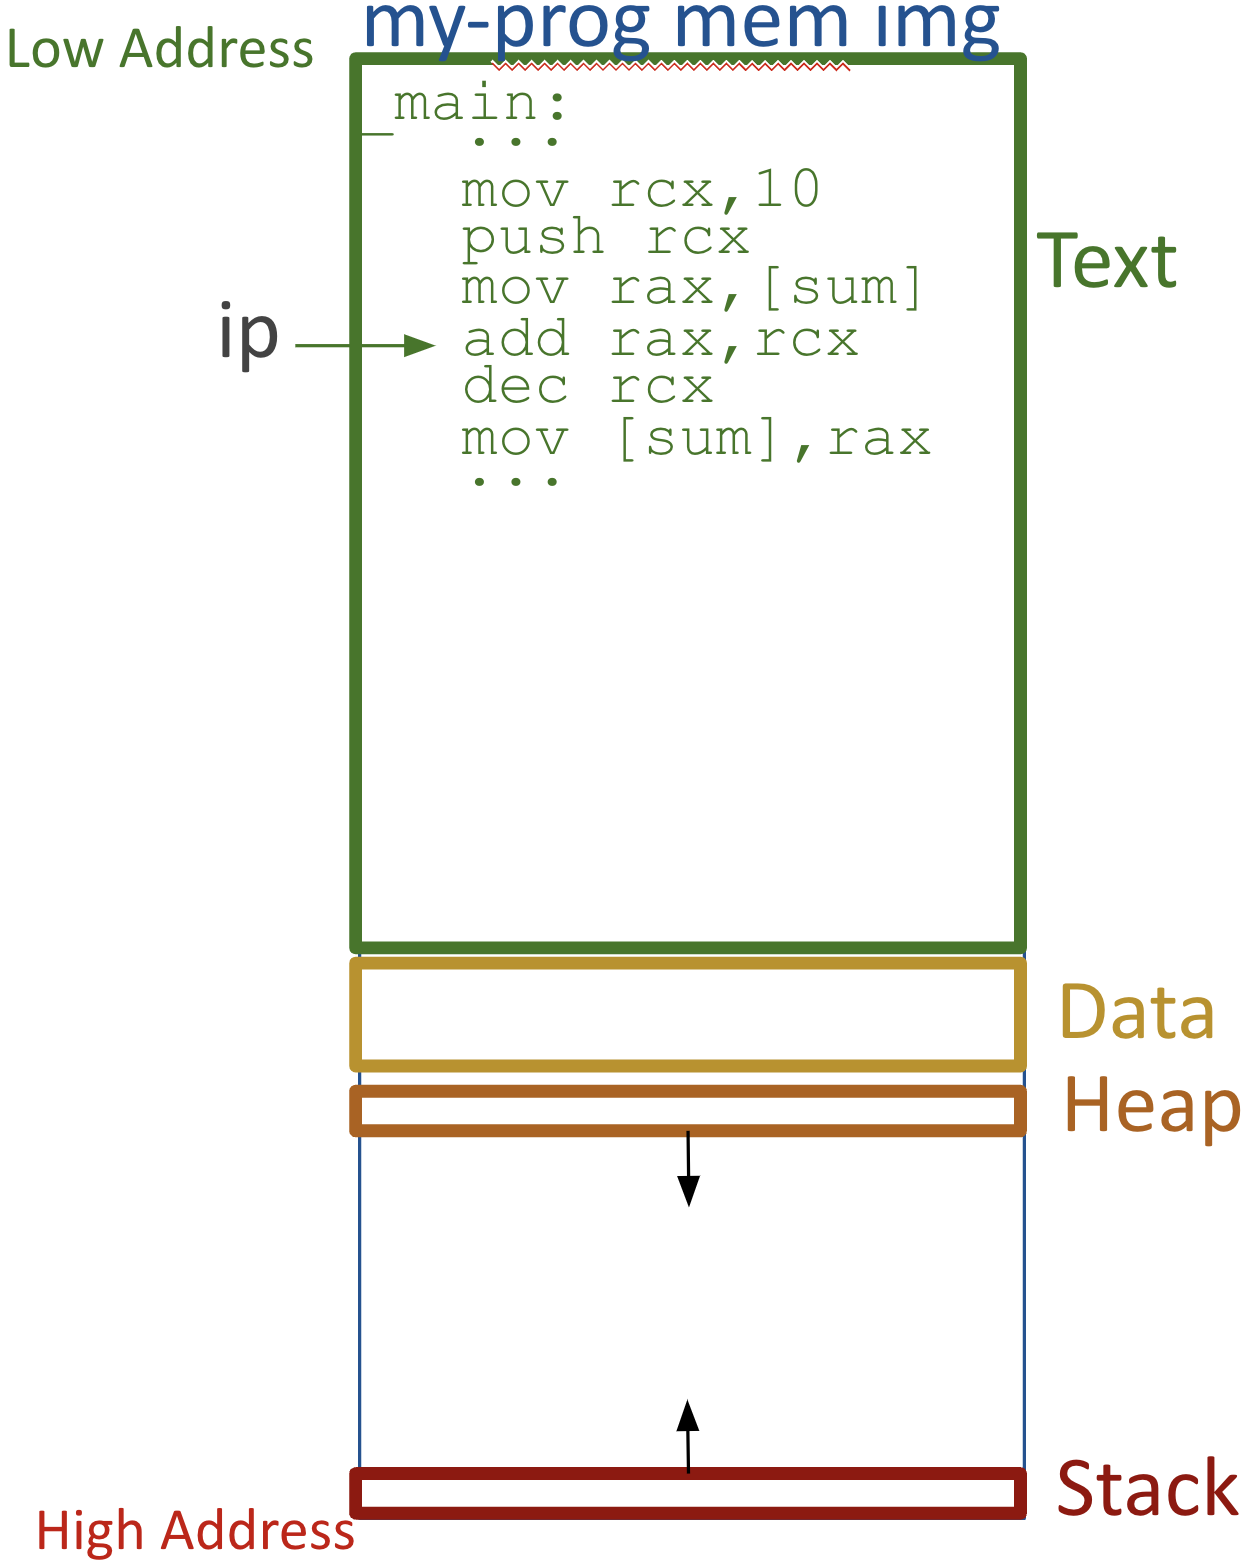
\includegraphics[width=1\textwidth]{images/mem_img.png}
    \end{center}
\end{minipage}\\[5px]
\hrule
\vspace{2px}
\begin{minipage}[htp]{1\textwidth}\vspace{5px}
    \noindent\textbf{Limited Direct Execution.} OS design allowing user programs to execute instructions directly on the CPU, with restrictions.
    \begin{itemize}[noitemsep,nolistsep,topsep=-10px,partopsep=0pt,parsep=0pt]
        \item[-] \textbf{Goal:} Maximize performance while maintaining control and protection.
        \item[-] \textbf{User Code Execution:} CPU runs user programs natively (not emulated) in \textbf{user mode}.
        \item[-] \textbf{OS Control:} OS retains control over hardware via \textbf{privileged instructions} and mode switching.
    \end{itemize}
    \vspace{15px}
    \noindent\textbf{User Mode vs Kernel Mode.} Two CPU execution modes stored as a state bit in a protected CPU register (0 = user mode, 1 = kernel mode) controlling access to hardware and instructions.
    \begin{itemize}[noitemsep,nolistsep,topsep=-10px,partopsep=0pt,parsep=0pt]
        \item[-] \textbf{User Mode:} Restricted. User code cannot execute privileged instructions or directly access hardware/memory management.
        \item[-] \textbf{Kernel Mode:} Mode in which is ran a central part of the operating system, the \textbf{Kernel}.
        \item[-] \textbf{Switching:} A transition from user mode to kernel mode is triggered by:
        \begin{itemize}[noitemsep,nolistsep]
            \item System Calls (e.g., file I/O, memory allocation)
            \item Hardware Interrupts (keyboard, timer,\dots)
            \item Software Traps (divide-by-zero, invalid memory access), \\
            \textit{If an exception happens in kernel mode, an internal routine is called but no mode switch occurs.}
        \end{itemize}
        After handling the event, the OS switches the CPU back to user mode to resume application execution.
    \end{itemize}\vspace{15px}
    \noindent\textbf{Privileged Instructions.} CPU instructions that can only execute in \textbf{kernel mode}. If attempted in user mode, the CPU raises a trap to the OS. Prevent user programs from interfering with other processes or the OS.\\
    \textbf{To do something that requires high privilege, a thread makes a \textbf{syscall}, invoking the kernel.} \\[-4px]
    \hrule
    \vspace{4px}
    \noindent\textbf{Exception/trap - synchronous signal.} The CPU itself raises an exception/trap. \\
    \noindent\textbf{Interrupt - asynchronous signal.} Some external entity raises an interrupt. If an external entity needs attention, it raises an \textbf{interrupt}, invokes the kernel. \\
    \noindent\textbf{Even if nothing external needs attention, the timer interrupt regularly invokes the kernel to run the \textbf{OS scheduler}.} \\[-5px]
    \end{minipage}
\end{minipage}
\hspace{2px}
\vline
\hspace{2px}
\begin{minipage}[htp]{0.5\textwidth}
\begin{minipage}[htp]{1\textwidth}
\noindent\textbf{Thread.} The smallest unit of CPU execution within a process. Multiple threads can exist within one process.
\begin{itemize}[noitemsep,nolistsep,topsep=-10px,partopsep=0pt,parsep=0pt]
    \item[-] \textbf{Memory:} Shares the parent process's virtual address space:
    \begin{itemize}[noitemsep,nolistsep,topsep=-10px,partopsep=0pt,parsep=0pt]
        \item[-] Shared: Code (text), heap, global/static data, open files.
        \item[-] Private: Each thread has its own stack (for local variables and function calls).
    \end{itemize}
    \item[-] \textbf{Execution context (per thread), values of all the CPU registers 
    at the \emph{last moment} the thread was running:}
    \begin{itemize}[noitemsep,nolistsep,topsep=-10px,partopsep=0pt,parsep=0pt]
        \item[-] \textbf{Instruction Pointer (IP) / Program Counter (PC):} Physical register pointing to the next instruction.Private per thread.
        \item[-] \textbf{Stack Pointer (SP):} Points to the top of the thread's private stack.
        \item[-] \textbf{General-purpose Registers:} Include temporary registers (e.g., RAX, RBX), status, and flags. \textbf{All private per thread.}
        \item[-] \textbf{Thread ID (TID).} The Thread ID is unique within a process, but not necessarily system-wide, assigned and tracked by the OS.\\
        \begin{minipage}[htp]{0.5\textwidth}
        \item[-] \textbf{Status:} OS tracks each thread's status (Running, Ready, Blocked).
        \item[-] \textbf{Virtualization:} Each thread has the illusion it exclusively occupies the CPU.
        \item[-] \textbf{Context switching:} OS saves/restores full register set (IP, SP, general-purpose regs). The CPU switches from one thread to another. Thread switches are faster than process switches.
        It saves to memory the CPU context of the current thread; it restores from memory the CPU context of the new thread.
        \item[-] \textbf{Thread management:} A main thread may create and manage others. In some models, a dedicated manager thread exists.
        \end{minipage}
        \hspace{-10px}
        \begin{minipage}[htp]{0.5\textwidth}
            \begin{center}
                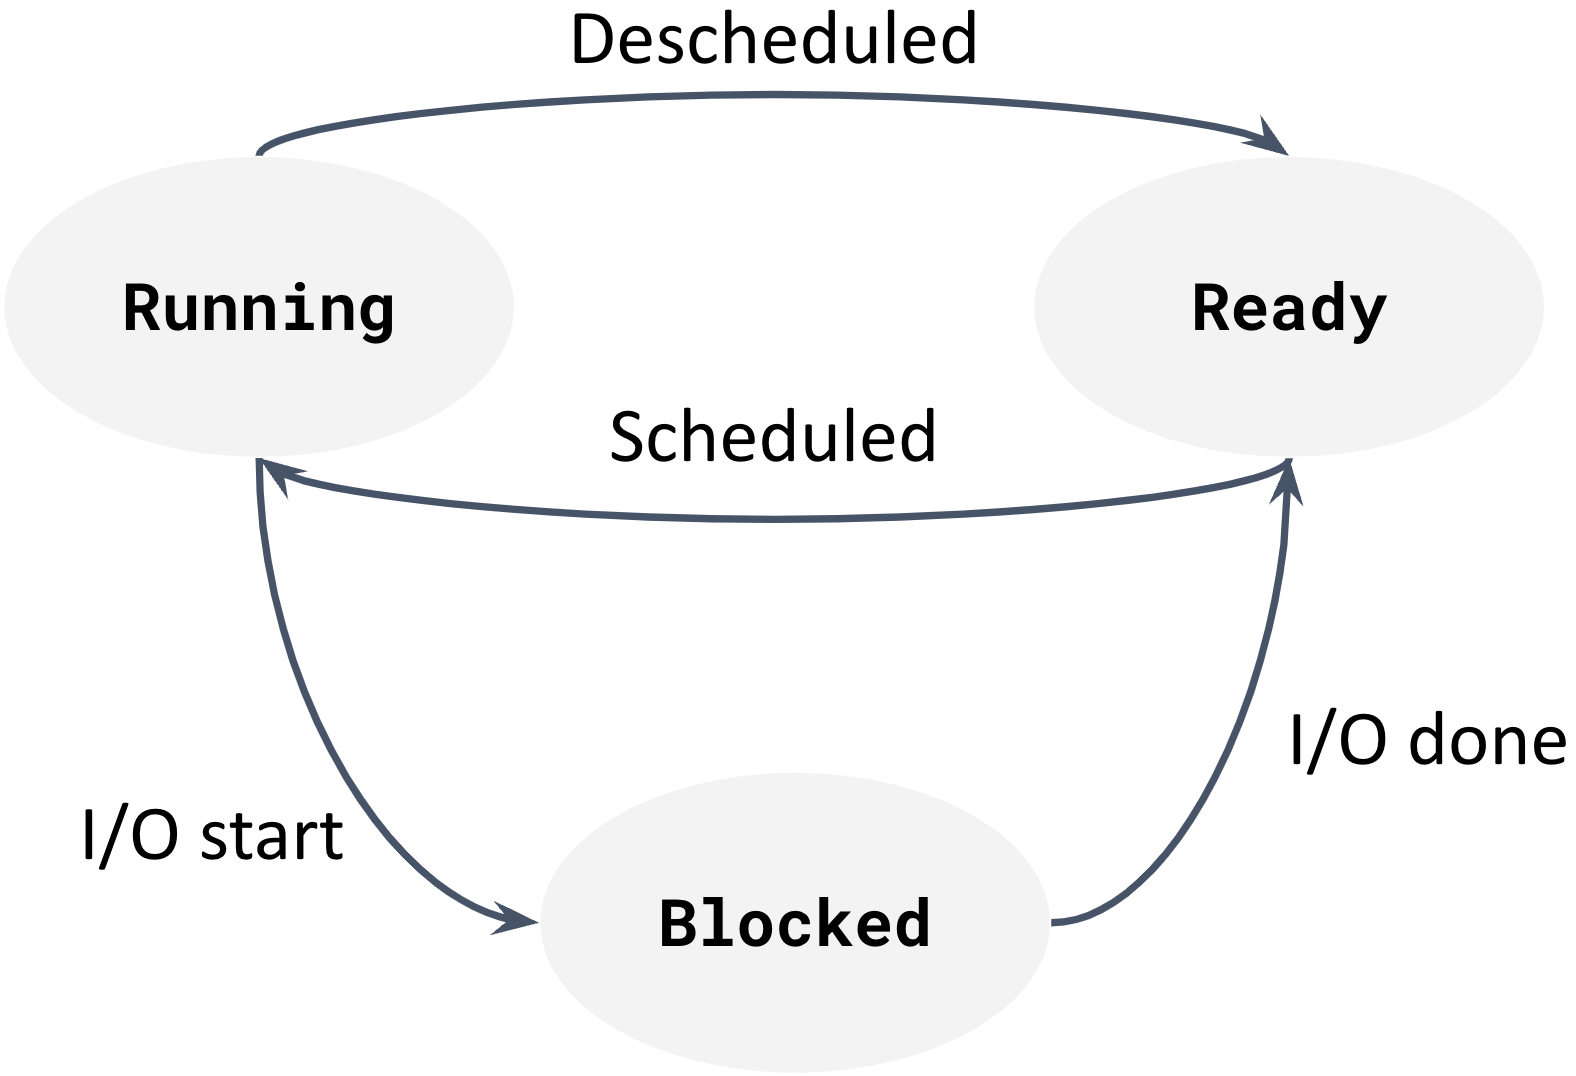
\includegraphics[width=0.85\textwidth]{images/thread_state.png}
            \end{center}
        \end{minipage}\\[2px]
    \item[-] \textbf{Managed by OS:} The OS kernel schedules threads individually and tracks them.
    \end{itemize}
\end{itemize}
\end{minipage}\\[5px]   
\hrule
\vspace{2px}
\begin{minipage}[htp]{1\textwidth}\vspace{5px}
    \noindent \textbf{OS Components.}
    \begin{itemize}[noitemsep,nolistsep,topsep=-10px,partopsep=0pt,parsep=0pt]  
        \item[-] \textbf{Kernel (core of the OS):} Loaded at boot, runs in \textbf{kernel mode}, and manages hardware, memory, processes, and system calls. It is the only part of the OS that runs in kernel mode.\\
        Three important routines inside of the kernel:
        \begin{itemize}[noitemsep,nolistsep,topsep=-10px,partopsep=0pt,parsep=0pt]  
            \item \textbf{Interrupt Handler or Interrupt Service Routine (ISR):} Handles interrupts from hardware devices.
            \item \textbf{Exception / Trap Handler:} Handles exceptions and traps from user programs.
            \item \textbf{System Call Handler:} Handles system calls from user programs.
        \end{itemize}
        \vspace{10px}
        The three routines use two tables (\textbf{Trap/Interrupt Table} and \textbf{System Call Table}) to resolve the event type to a specific memory address of the handler routine managing the event.
        \item[-] \textbf{Loader (part of the OS):} Prepares executables to run:
        \begin{itemize}[noitemsep,nolistsep,topsep=-10px,partopsep=0pt,parsep=0pt]  
            \item Loads program code/data into memory.
            \item Maps required libraries (e.g., libc).
            \item Sets up the process stack and heap.
            \item Places command-line arguments and environment variables on the stack.
            \item Sets the \texttt{\%rsp} (stack pointer) and \texttt{\%rdi} (argc), \texttt{\%rsi} (argv) registers so the program can access arguments.
            \item \textit{Because the kernel manages processes and initiates execution, it is responsible for placing arguments in registers so the loader (running in user mode) can access them.}
            \item Jumps to the program's entry point to begin execution in \textbf{user mode}.
        \end{itemize}
        \item[-] \textbf{User-level Programs:} Applications like shells, editors, browsers, etc. These are \textbf{part of the OS} but run entirely in \textbf{user mode}, relying on system calls to request kernel services.
        \item[-] \textbf{System Libraries:} Shared libraries (e.g., libc) used by user programs. Loaded and linked by the loader, but executed in user mode. Provide wrappers around system calls.
    \end{itemize}
    \end{minipage}
\end{minipage}\\[5px]
\hrule
\hspace{-20px}
\begin{minipage}[t]{0.4\textwidth}
    \textbf{fork()} — \textit{Clone the current process}
    \begin{enumerate}[noitemsep,nolistsep,topsep=-10px,partopsep=0pt,parsep=0pt]  
        \item The operating system creates a new process (child) by \\duplicating the calling process.
        \item The child initially shares all memory pages with the parent:\\
           - Pages are marked read-only and shared (Copy-On-Write).\\
           - If either process attempts to write to a page, it is copied privately for that process.
        \item The child also receives:\\
       - Duplicated file descriptors (pointing to the same open files). \\
       - Identical program counter and stack pointer.
        \item Returns:\\
        - In the parent process: the PID of the child.\\
        - In the child process: \texttt{0}.
        \item Both processes resume execution at the instruction following \texttt{fork()}.
    \end{enumerate}    
\end{minipage}
\begin{minipage}[t]{0.2\textwidth}
 \textbf{exec()} — \textit{Mutate the child into a new program}
    \begin{itemize}[noitemsep,nolistsep,topsep=-10px,partopsep=0pt,parsep=0pt]  
        \item Typically called by the child process immediately after \texttt{fork()}.
        \item Replaces the child’s memory space with a new program image.
        \item Stack, heap, code, and data segments are replaced.
        \item If successful: the new program starts execution from \texttt{main()}.
        \item If failed: \texttt{exec()} returns \texttt{-1}, child continues old code.
    \end{itemize}
\end{minipage}
\begin{minipage}[t]{0.2\textwidth}
 \textbf{exit()} — \textit{Terminate a process cleanly}
    \begin{itemize}[noitemsep,nolistsep,topsep=-10px,partopsep=0pt,parsep=0pt]  
        \item Frees system resources allocated to the process.
        \item Sends termination status to the parent.
        \item If main function of a program returns, \texttt{exit()} is implicitly called.
    \end{itemize}
\end{minipage}
\begin{minipage}[t]{0.21\textwidth}
 \textbf{wait()} — \textit{Wait for a child process to terminate}
    \begin{itemize}[noitemsep,nolistsep,topsep=-10px,partopsep=0pt,parsep=0pt]  
        \item Blocks the calling process until one of its child processes terminates.
        \item Returns the PID of the terminated child.
        \item If no child processes exist, it waits indefinitely.
    \end{itemize}
\end{minipage}
\newpage
\hspace*{-20px}
\begin{minipage}[htp]{0.5\textwidth}
\begin{minipage}[htp]{1\textwidth}
\noindent\textbf{Memory Management Unit (MMU) - Address Translation.}  \\
\textbf{Hardware component} managed by the \textbf{operating system} that translates \textbf{virtual addresses} into \textbf{physical addresses} using \textbf{per-process page tables}. \textbf{Each process has its own page table, and the currently active one is referenced in a special CPU register.} \\
\fbox{\begin{minipage}[htp]{1\textwidth}
\noindent\textbf{Translation Lookaside Buffer (TLB).} \\
\begin{minipage}[htp]{0.45\textwidth}
\small
A small, fast \textbf{cache inside the MMU} that stores recent \textbf{virtual-to-physical page mappings}. The TLB reduces the need to access the page table on every memory reference, significantly speeding up address translation.
\end{minipage}
\begin{minipage}[htp]{0.55\textwidth}
\begin{center}
    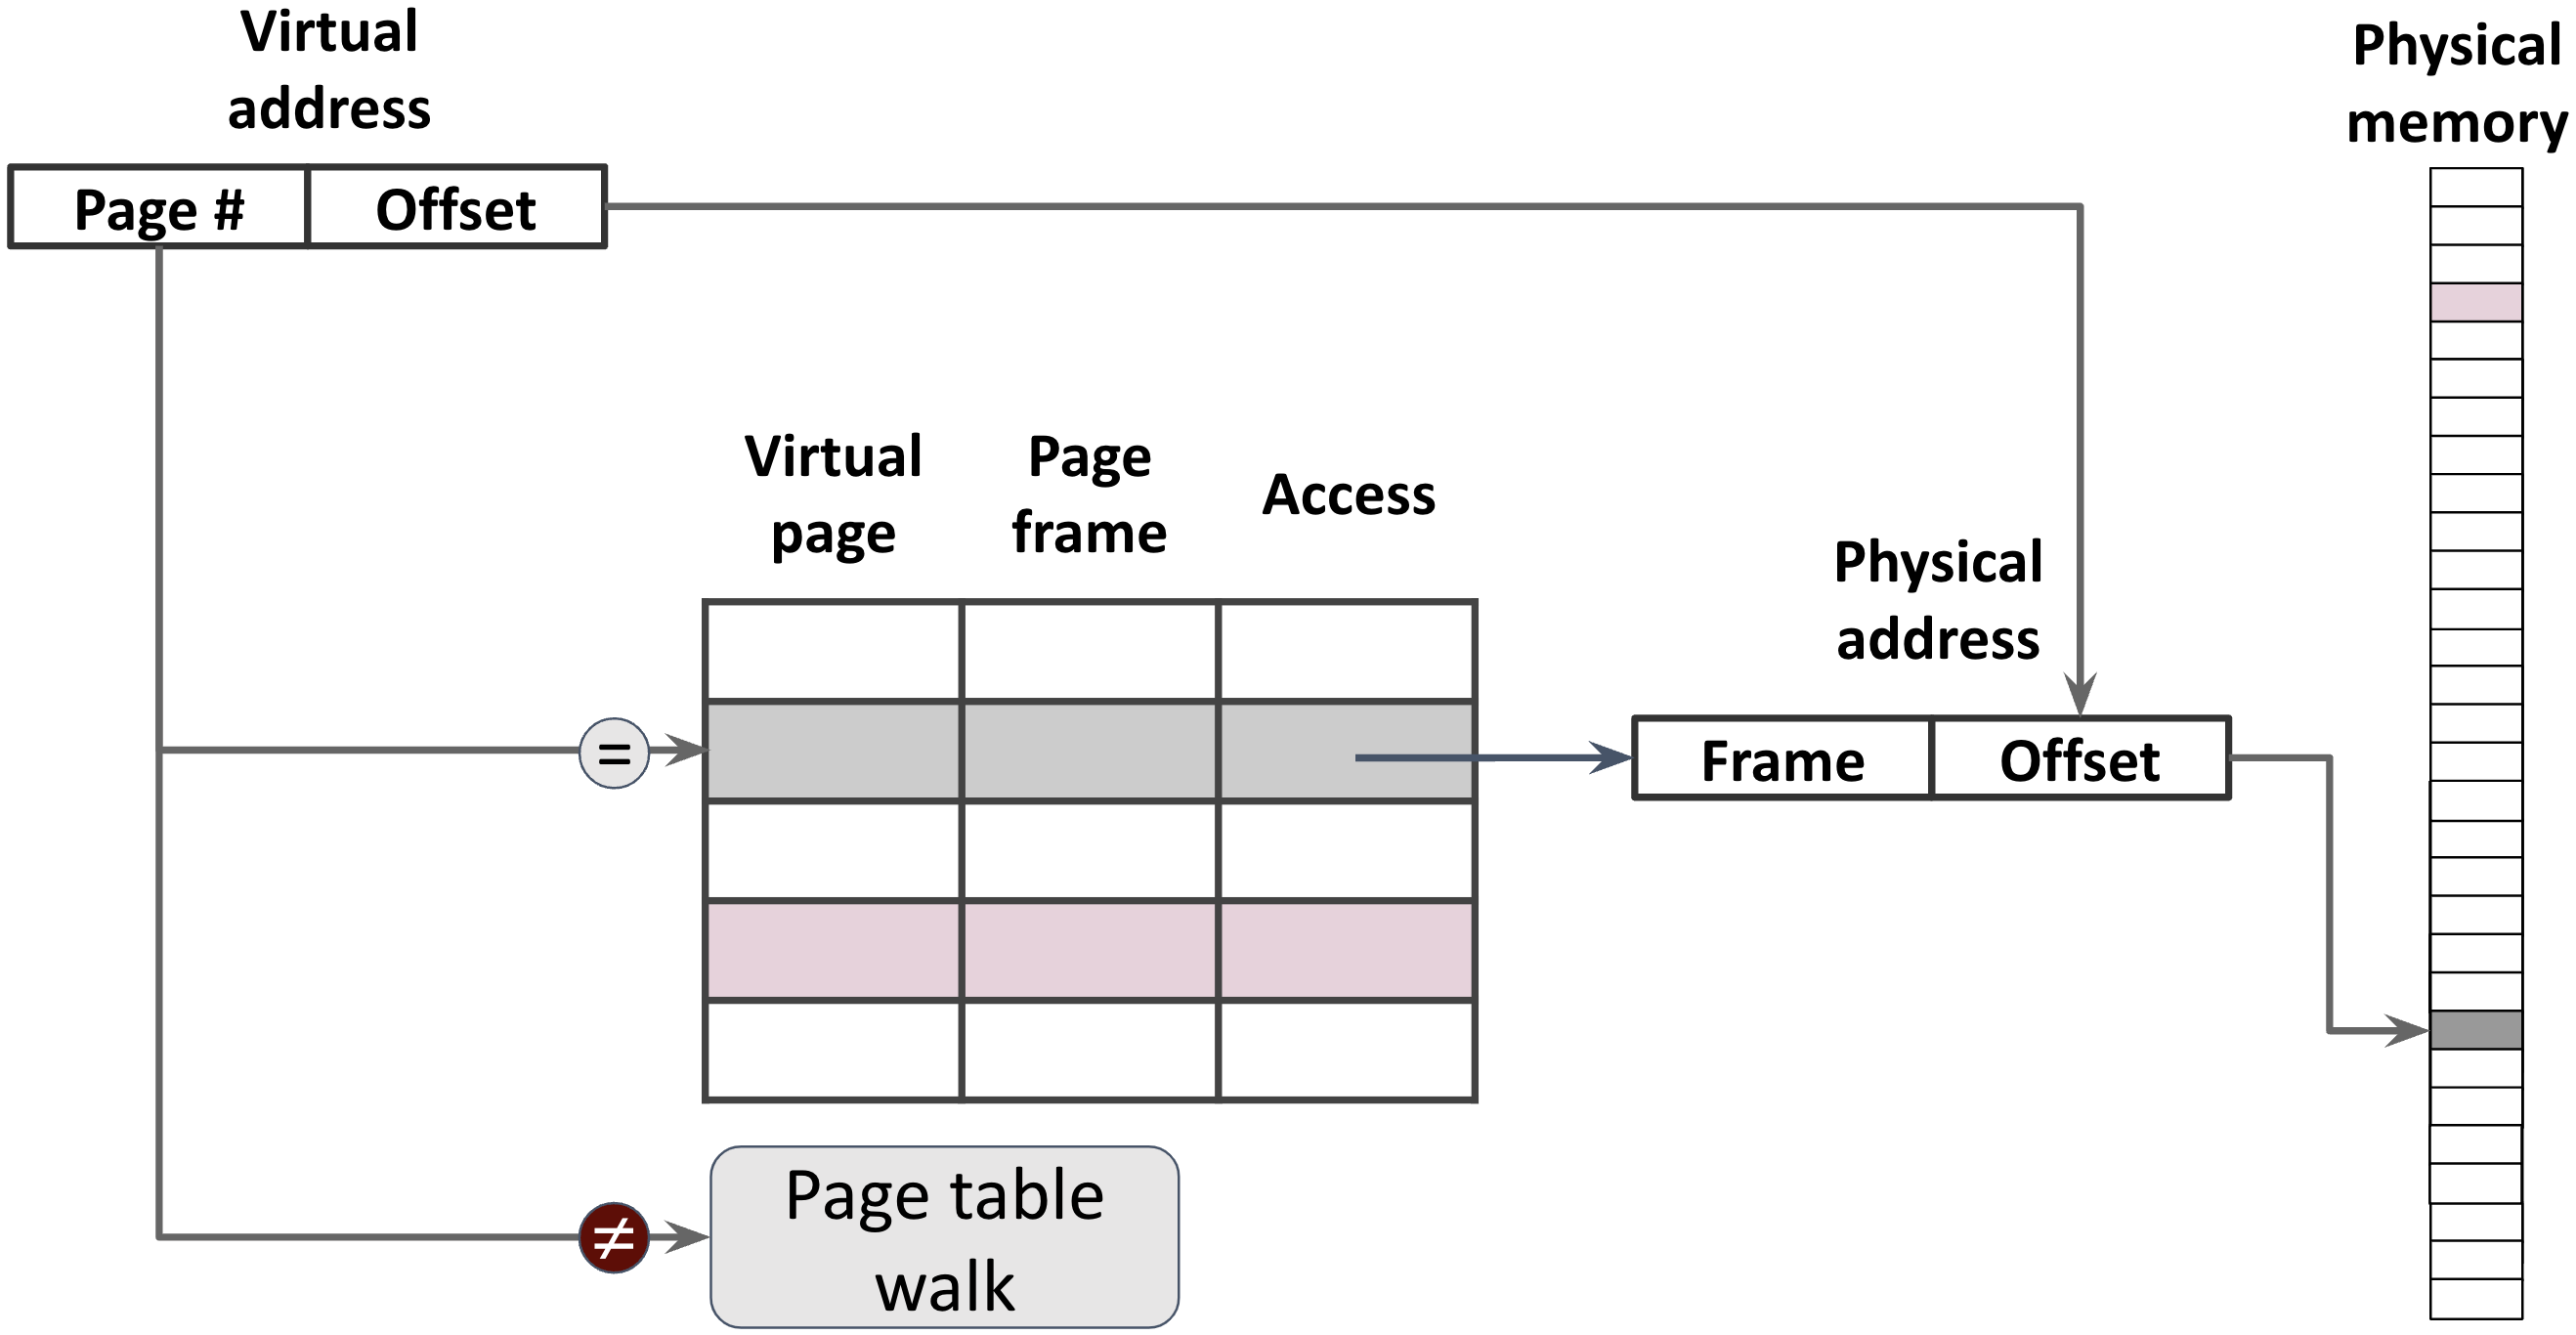
\includegraphics[width=1\textwidth]{images/tlb.png}
\end{center}
\end{minipage}
\end{minipage}}\\[2px]
    \noindent\textbf{Virtual Address Translation:}
    \begin{enumerate}[noitemsep,nolistsep,topsep=-10px,partopsep=0pt,parsep=0pt]
        \item The \textbf{CPU executes an instruction} (e.g., \texttt{load}, \texttt{store}, or \texttt{fetch}) that references a memory location using a \textbf{virtual address}.
        \item The \textbf{MMU extracts} the \textbf{virtual page number (VPN)} and \textbf{page offset} from the virtual address.
        \item The MMU first checks the \textbf{TLB} for a cached translation of the VPN.
        \item \textbf{If the translation is found in the TLB (TLB hit):}
        \begin{enumerate}[noitemsep,nolistsep,topsep=0pt]
            \item The corresponding \textbf{physical frame number} is retrieved directly.
        \end{enumerate}
\item \textbf{If the translation is not found (TLB miss $\rightarrow$ page table walk):}
    \begin{enumerate}[noitemsep,nolistsep,topsep=0pt]
        \item The MMU uses the active \textbf{page table} to look up the VPN and obtain the PFN.
        \item The new mapping is inserted into the TLB for future accesses.
    \end{enumerate}
    \item \textbf{If the page table entry is invalid or \texttt{present = 0} (page fault):}
    \begin{enumerate}[noitemsep,nolistsep,topsep=0pt]
        \item The CPU triggers a \textbf{trap into the OS kernel}.
        \item The \textbf{page fault handler} in the OS's \textbf{memory management subsystem} is invoked.
        \item The handler checks whether the page is:
        \begin{enumerate}[noitemsep,nolistsep,topsep=0pt]
            \item \textbf{Never allocated before} $\rightarrow$ allocate a new physical page and zero-initialize it.
            \item \textbf{Swapped out to disk} $\rightarrow$
            \begin{enumerate}[noitemsep,nolistsep,topsep=0pt]
                \item Check the \textbf{swap cache} for the page.
                \item If found in the swap cache, use the cached page directly.
                \item If not in the cache, read the page from the \textbf{swap space} on disk into a free physical frame, and insert it into the swap cache.
            \end{enumerate}
        \end{enumerate}
        \item The newly loaded or allocated page is mapped in the page table, and \texttt{present} is set to \texttt{1}.
        \item The TLB entry for the VPN is updated if needed.
        \item The faulting instruction is retried.
    \end{enumerate}
    \item The final \textbf{physical address} is then used to \textbf{access RAM}.
\end{enumerate}
\vspace{1em}
\noindent\textbf{Swapping}\\
Transfer of memory pages between physical RAM and disk-based swap space to free up RAM.\\
- \textbf{Swap Space} Disk region reserved for evicted pages; holds non-resident memory to extend usable RAM.\\ 
- \textbf{Swap Cache} In-memory buffer of recently swapped-out pages; enables fast lookup and avoids redundant disk I/O during swap-in. \\
-\noindent\textbf{Swap-Outs:}
\begin{enumerate}[noitemsep,nolistsep,topsep=-5px,partopsep=0pt,parsep=0pt]
    \item The OS detects that the number of free physical pages has fallen below a predefined threshold.
    \item A background kernel thread is triggered to reclaim memory.
    \item The kernel scans memory to identify candidate pages for eviction, typically using an aging or Least Recently Used algorithm.
    \item A candidate page is selected if:
    \begin{enumerate}[noitemsep,nolistsep,topsep=0pt]
        \item It is not currently in use (i.e., not recently accessed),
        \item It is not locked, pinned, or shared with kernel-critical structures.
    \end{enumerate}
    \item If the selected page is dirty (i.e., has been modified), its contents are written to the swap space on disk.
    \item The page is inserted into the \textbf{swap cache} so it can be quickly retrieved if needed again.
    \item The page table entry is updated: \texttt{present = 0}, and the swap location is recorded.
    \item The physical frame is freed and returned to the pool of available memory.
\end{enumerate}
\end{minipage}\\
\vspace{3px}
\hrule
\vspace{3px}
\begin{minipage}[htp]{1\textwidth}

    \noindent\textbf{CPU Cache.} \\
    The \textbf{CPU cache} is a small, fast memory located on or near the processor that stores copies of frequently accessed data from main memory (RAM). Its purpose is to reduce memory access latency and improve overall performance by exploiting \textbf{temporal} and \textbf{spatial locality}.\\
    \noindent\textbf{Cache Levels:}
    \begin{itemize}[noitemsep,topsep=0pt]
        \item \textbf{L1 Cache (Level 1):} The smallest and fastest cache, located right on the CPU core. 64 KB, but takes $< 1 nsec$ to access.
        \item \textbf{L2 Cache (Level 2):} Larger and slightly slower than L1, still located on the CPU core.256-512 KB, takes $< 4 nsec$ to access.
        \item \textbf{L3 Cache (Level 3):} Shared among multiple cores, larger but slower than L1 and L2. Located on the CPU die. 6-32 MB, takes $10s \;of \;nsec$ to access.  
    \end{itemize}
    \noindent\textbf{Hierarchy Behavior:} \\
    Caches form a \textbf{hierarchy}: the CPU checks L1 first, then L2, then L3, and finally main memory if needed. This optimizes for latency and hit rate.
    \end{minipage}
\end{minipage}
\hspace{5px}
\vline
\hspace{5px}
\begin{minipage}[htp]{0.48\textwidth}
\vspace*{-10px}
\begin{minipage}[htp]{1\textwidth}
\noindent\textbf{Paging.} \\
Paging divides virtual memory into fixed-size \textbf{pages}, mapped to physical \textbf{frames} via a \textbf{page table}. It avoids \textbf{ext. fragmentation}, but may cause \textbf{internal fragmentation} if a page is only partially used.\\

\noindent\textbf{Address Representation.} \\
\textbf{Virtual Addresss Size is not always equal to Physical Address Size!}\\ 
Let $m$ be the number of bits in the \textbf{virtual address} (i.e., $m = \log_2(\text{virtual address space size})$). \\
This also corresponds to the number of bits required to uniquely address every byte in the virtual memory. If the virtual memory consists of $2^k$ pages and each page is $2^n$ bytes, then the total virtual address space is $2^k \times 2^n = 2^m$ bytes, and thus $m = k + n$.
\begin{center}
    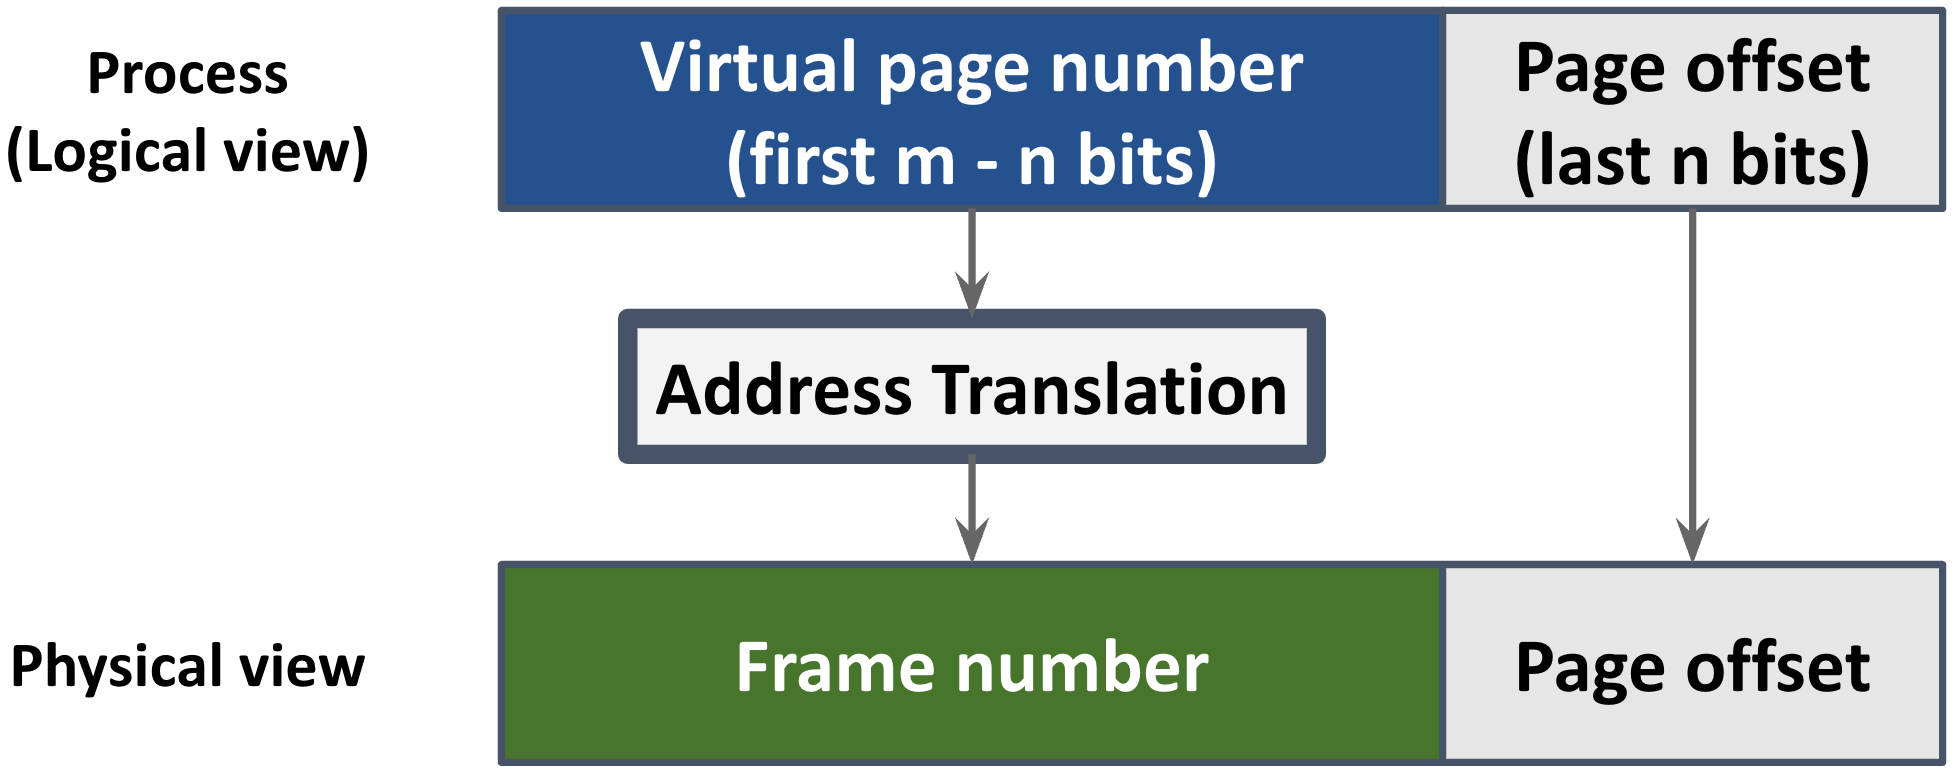
\includegraphics[width=0.65\textwidth]{images/paging.png}
\end{center}
A virtual address is split into:
\begin{itemize}[noitemsep,topsep=0pt]
    \item[-] \textbf{Offset} ($n$ bits): identifies a byte within a page of size $2^n$ bytes, where $n = \log_2(\text{page size})$.
    \item[-] \textbf{Virtual Page Number (VPN)} ($m - n$ bits): selects the page entry from the page table.
\end{itemize}
\end{minipage}\\[2px]
\hrule
\vspace{3px}
\begin{minipage}[htp]{1\textwidth}
    \noindent\textbf{Page Table.} \\
    A process's \textbf{page table} maps each \textbf{Virtual Page Number (VPN)} to a \textbf{Physical Frame Number (PFN)}. The page table is indexed by the VPN and stores \textbf{Page Table Entries (PTEs)}.\\[5px]
    \noindent\textbf{Linear Page Table.} \\
    A single-level table with $2^{m - n}$ entries. Each VPN directly indexes a PTE. Simple but potentially large: $\Rightarrow$ Table size = $2^{m - n} \times \text{PTE size}$ (may span multiple memory pages).\\[5px]
    \noindent\textbf{PTE Content (Typical Metadata Bits):}
    \begin{itemize}[noitemsep,topsep=0pt]
        \item[-] \textbf{Present bit (P):} Valid address translation exists
        \item[-] \textbf{Protection bits (R/W/X):} Read, write, execute permissions
        \item[-] \textbf{User/Supervisor (U/S):} Access control (user vs. kernel)
        \item[-] \textbf{Dirty bit (D):} Set if the page has been modified
        \item[-] \textbf{Access/Reference bit (A):} Set on access; used in replacement policies
    \end{itemize}
    \vspace{5px}
    \noindent\textbf{Multi-Level Page Tables.} \\
    Used to reduce memory overhead. Split the VPN into multiple parts to form a tree-like hierarchy. The \textbf{offset} remains the last $n = \log_2(\text{page size})$ bits of the address.\\
    \noindent\textbf{General Breakdown (Multi-Level Paging):}
    \begin{center}
    $\text{Virtual Address Size} = m = \sum k_i + n$
    \end{center}
    \vspace{-5px}
    where:
    \begin{itemize}[noitemsep,topsep=0pt]
        \item[-] $n = \log_2(\text{page size})$: offset bits
        \item[-] $k_i$: number of bits used at each level of the page table
    \end{itemize}
    \vspace{5px}
    \noindent\textbf{Two-Level Page Table:}
\begin{center}$
    \text{VPN} = \underbrace{\text{Level 1 index}}_{k_1} \ \|\ \underbrace{\text{Level 2 index}}_{k_2}, \quad k_1 + k_2 = m - n
$\end{center}\vspace{-10px}
    \begin{itemize}[noitemsep,topsep=0pt]
        \item Level 1 index ($k_1$ bits): selects the \textbf{page directory entry (PDE)}
        \item Level 2 index ($k_2$ bits): selects the \textbf{page table entry (PTE)} from the second-level table
    \end{itemize}
\vspace{5px}
    \noindent\textbf{Three-Level Page Table:}
\begin{center}$
    \text{VPN} = \underbrace{\text{L1 index}}_{k_1} \ \|\ \underbrace{\text{L2 index}}_{k_2} \ \|\ \underbrace{\text{L3 index}}_{k_3}, \quad k_1 + k_2 + k_3 = m - n
$\end{center}\vspace{-10px}
    \begin{itemize}[noitemsep,topsep=0pt]
        \item Level 1 index ($k_1$ bits): selects \textbf{first-level page directory}
        \item Level 2 index ($k_2$ bits): selects \textbf{second-level directory/table}
        \item Level 3 index ($k_3$ bits): selects the final \textbf{PTE}
    \end{itemize}

    \noindent\textbf{Bit Allocation in Multi-Level Page Tables:} \\
    The VPN portion ($m - n$ bits) is divided into $L$ parts ($k_1 + k_2 + \dots + k_L = m - n$), one per level.
    \begin{itemize}[noitemsep,topsep=0pt]
        \item \textbf{Bit division is not necessarily even.} Systems may assign more bits to higher levels.
        \item If uneven, \textbf{last levels (closer to the leaf)} typically receive \textbf{fewer bits} (fewer entries).
        \item Each level $i$ contains $2^{k_i}$ entries, indexing the next level or the final PTE.
    \end{itemize}
\end{minipage}\\[3px]
\hrule
\vspace{3px}
\noindent\textbf{Segmentation.} \\
Segmentation divides memory into variable-sized \textbf{logical segments} (e.g., code, data, stack), each with a base and limit. It aligns with program structure and supports segment-level protection, but suffers from \textbf{ext. fragmentation} due to variable-sized allocations.
\end{minipage}
\newpage
\hspace{-20px}
%%%%%%%%%%%%%%%%%%%%%%%% FS API %%%%%%%%%%%%%%%%%%%%%%%%%%%%%%%%
\begin{minipage}[htp]{0.5\textwidth}
    \noindent\textbf{File System API.} Kernel provides access to files and directories through system calls. Files are represented using \textbf{File Descriptors (FDs)} — integers indexing into a \textbf{per-process FD table}.

    \begin{itemize}[noitemsep,nolistsep,topsep=-10px,partopsep=0pt,parsep=0pt]
        \item[-] \textbf{File Descriptor:} Non-negative int returned by \texttt{open()}. Index into the process’s FD table.
        \item[-] \textbf{Open File Description (OFD):} Kernel object holding metadata like file offset, mode, and inode reference.
        \item[-] \textbf{Per-Process Table:} Each process has its own FD table mapping integers to OFDs.
        \item[-] \textbf{Reserved FDs:} 0 = \texttt{stdin}, 1 = \texttt{stdout}, 2 = \texttt{stderr}.
        \item[-] \textbf{FD Allocation:} \texttt{open()} returns the lowest unused FD.
    \end{itemize}

    \vspace{15px}
    \noindent\textbf{Common FS System Calls.} Core interface for file I/O and positioning.
    \begin{itemize}[noitemsep,nolistsep,topsep=-10px,partopsep=0pt,parsep=0pt]
        \item[-] \texttt{open(path, flags, mode):} Open file, return FD. \\Flags: \texttt{O\_RDONLY}, \texttt{O\_WRONLY}, \texttt{O\_RDWR}, \texttt{O\_CREAT}, \texttt{O\_TRUNC}.
        \item[-] \texttt{read(fd, buf, count):} Read up to \texttt{count} bytes from FD into buffer.
        \item[-] \texttt{write(fd, buf, count):} Write up to \texttt{count} bytes from buffer to FD.
        \item[-] \texttt{lseek(fd, offset, whence):} Move file offset. \texttt{SEEK\_SET} = from start, \texttt{SEEK\_CUR} = from current, \texttt{SEEK\_END} = from end.
        \item[-] \texttt{unlink(path):} Remove (delete) a file. File is deleted once no processes have it open.
        \item[-] \texttt{fsync(fd):} Flush all modified file data and metadata to disk.
        \item[-] \texttt{fstat(fd, \&statbuf):} Get metadata about file referred to by FD (size, mode, timestamps, etc.).
    \end{itemize}    
    \vspace{15px}
    \begin{minipage}[t]{0.49\textwidth}
        \noindent\textbf{File Internals.} A file consists of two main components: \textbf{data} and \textbf{metadata}.
        \begin{itemize}[noitemsep,nolistsep,topsep=-8px,partopsep=0pt,parsep=0pt]
            \item[-] \textbf{Data:} Actual user content, stored in data blocks.
            \item[-] \textbf{Metadata:} Stored in the inode:
            \begin{itemize}[noitemsep,nolistsep]
                \item[-] Owner, permissions, timestamps
                \item[-] File size, type, and block pointers
                \item[-] Device ID and inode number
            \end{itemize}
            \item[-] \textbf{Inode:} Kernel-managed structure that holds file metadata and pointers to data blocks.
            \item[-] \textbf{Filename:} Not stored in the inode. Stored in directory entries.
            \item[-] \textbf{Uniqueness:} File is uniquely identified by (device, inode).
            \item[-] \textbf{Allocation:} Inodes are created and managed by the file system.
        \end{itemize}
    \end{minipage}
    \hfill
    \begin{minipage}[t]{0.49\textwidth}
        \noindent\textbf{Directory Internals.} A directory is a \textbf{special file} used to organize and reference files.
            - \textbf{Structure:} Stored like a regular file, but marked with a directory flag in its inode. \\
            - \textbf{Content:} Contains a list of entries:\\ 
            - Each entry is a \texttt{filename $\rightarrow$ inode number} mapping\\
            - \textbf{Function:} Maps human-readable names to inodes.\\
            - \textbf{Permissions:} Govern ability to read entries, traverse, or modify structure.\\
            - \textbf{Traversal:} Used in path resolution to step through the hierarchy.\\
            - \textbf{Isolation:} \textbf{Normal processes cannot write directly to directories as a file (writing arbitrary bytes is not allowed).}
    \end{minipage}\\
    \begin{minipage}[t]{0.49\textwidth}
    \noindent\textbf{Path Resolution, Step-by-Step.} \\
    Converting a pathname to a target inode involves directory traversal.
    \begin{enumerate}[noitemsep,nolistsep,topsep=-10px,partopsep=0pt,parsep=0pt]
        \item Begin at root (\texttt{/}) or current working directory.
        \item Parse each path component left to right.
        \item For each component, look up entry in current directory: \texttt{filename → inode number}.
        \item Follow inode to next directory or target file.
        \item Final inode is cached in the file descriptor table for future access.
    \end{enumerate}
\end{minipage}
\hfill
\begin{minipage}[t]{0.49\textwidth}
    \hrule
    \vspace{5px}
    \noindent\textbf{Mount Point.} \\
Directory where a filesystem is attached to the global namespace. Root filesystem is mounted at \texttt{/}.\\
\textbf{mount command.} \\
Attach filesystem to directory (mount point).\\
\texttt{mount [device] [dir]} \\ mount device at dir.\\
\textbf{df command.} \\
Display filesystem disk usage.\\
\texttt{df --} report filesystem disk usage.\\
\end{minipage}\\[5px]
\noindent\textbf{Partition.} \\
Linear view of persistent storage: sequence of \texttt{N} blocks, indexed \texttt{0 to N-1}. \\
\begin{minipage}[t]{0.4\textwidth}
    \noindent\textbf{Inode.} \\
    Filesystem structure representing a file. Each inode stores:
    \begin{itemize}[noitemsep,topsep=0pt]
        \item File type and permissions
        \item Owner UID / GID
        \item File size
        \item Timestamps (created, modified, accessed)
        \item Pointers to data blocks
        \item Link count (number of directory references)
    \end{itemize}
\end{minipage}
\begin{minipage}[t]{0.55\textwidth}
\noindent\textbf{Block Usage.}
\begin{itemize}[noitemsep,topsep=0pt]
    \item[-] \textbf{Data blocks} — store file contents.
    \item[-] \textbf{Metadata blocks} — store filesystem structures.
    \item[-] \textbf{Boot block} — code for booting (block 0).
    \item[-] \textbf{Superblock} — global File System metadata:
        \begin{itemize}[noitemsep,topsep=0pt]
            \item number of inodes, number of data blocks
            \item Inode table location
            \item Free inode/data block management
        \end{itemize}
\end{itemize}
\end{minipage}\\[2px]
\begin{minipage}[htp]{1\textwidth}
\noindent\textbf{Block Types.}\\
\hspace*{-35px}
\begin{minipage}[t]{0.5\textwidth}
\begin{itemize}[noitemsep,topsep=0pt]
    \item[] (I) \textbf{Inode Block} — contains array of inodes (e.g., 16 inodes/block at 256B each).
    \item[] (D) \textbf{Data Block} — holds actual file content (user data).
    \item[] (i)/(d) \textbf{Bitmap Blocks} — tracks used/free inodes and data blocks (free list).
\end{itemize}
\end{minipage}%
\hspace*{-10px}
\begin{minipage}[t]{0.5\textwidth}
\begin{itemize}[noitemsep,topsep=0pt]
    \item[(S)] \textbf{Superblock} — global FS metadata:
        \begin{itemize}[noitemsep,topsep=0pt]
            \item Total inodes and data blocks
            \item Inode table start block
            \item Bitmap locations
            \item FS state (clean, dirty)
        \end{itemize}
    \item[(B)] \textbf{Boot Block} — bootloader code; block 0 of partition.
\end{itemize}
\end{minipage}
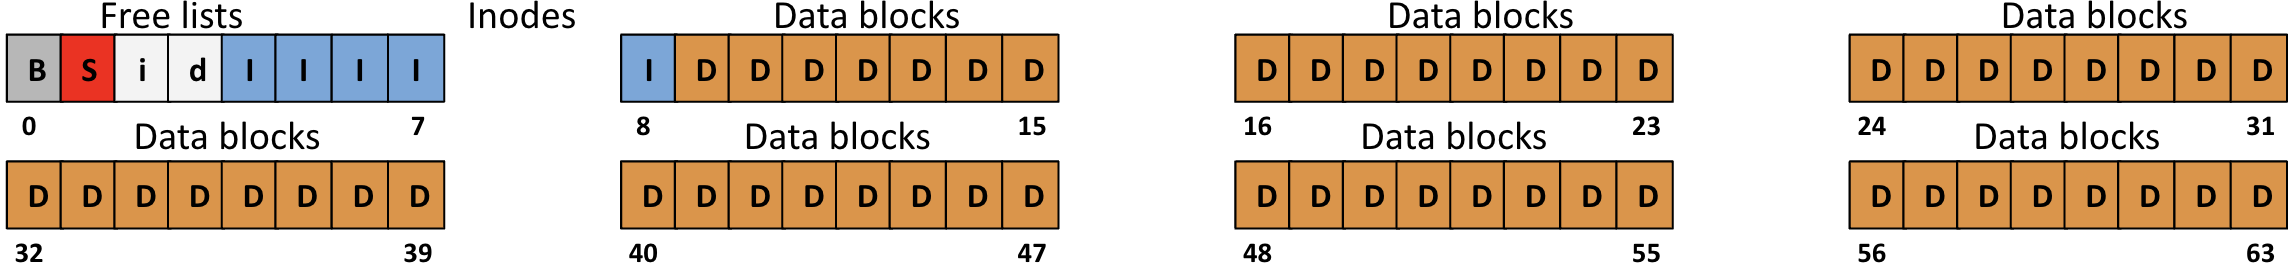
\includegraphics[width=1\textwidth]{images/blocks.png}
\end{minipage}
\end{minipage}
\small
\begin{minipage}[htp]{0.5\textwidth}

    \begin{minipage}[htp]{0.45\textwidth}
    \textbf{Links.} Multiple names can refer to files using links.\\
- \textbf{Hard Link:} Maps a file name directly to the \textbf{same inode} as the original file, deleting one's file name does not remove the actual data as long as another link still exists.
    \end{minipage}
    \hfill
    \begin{minipage}[htp]{0.55\textwidth}
        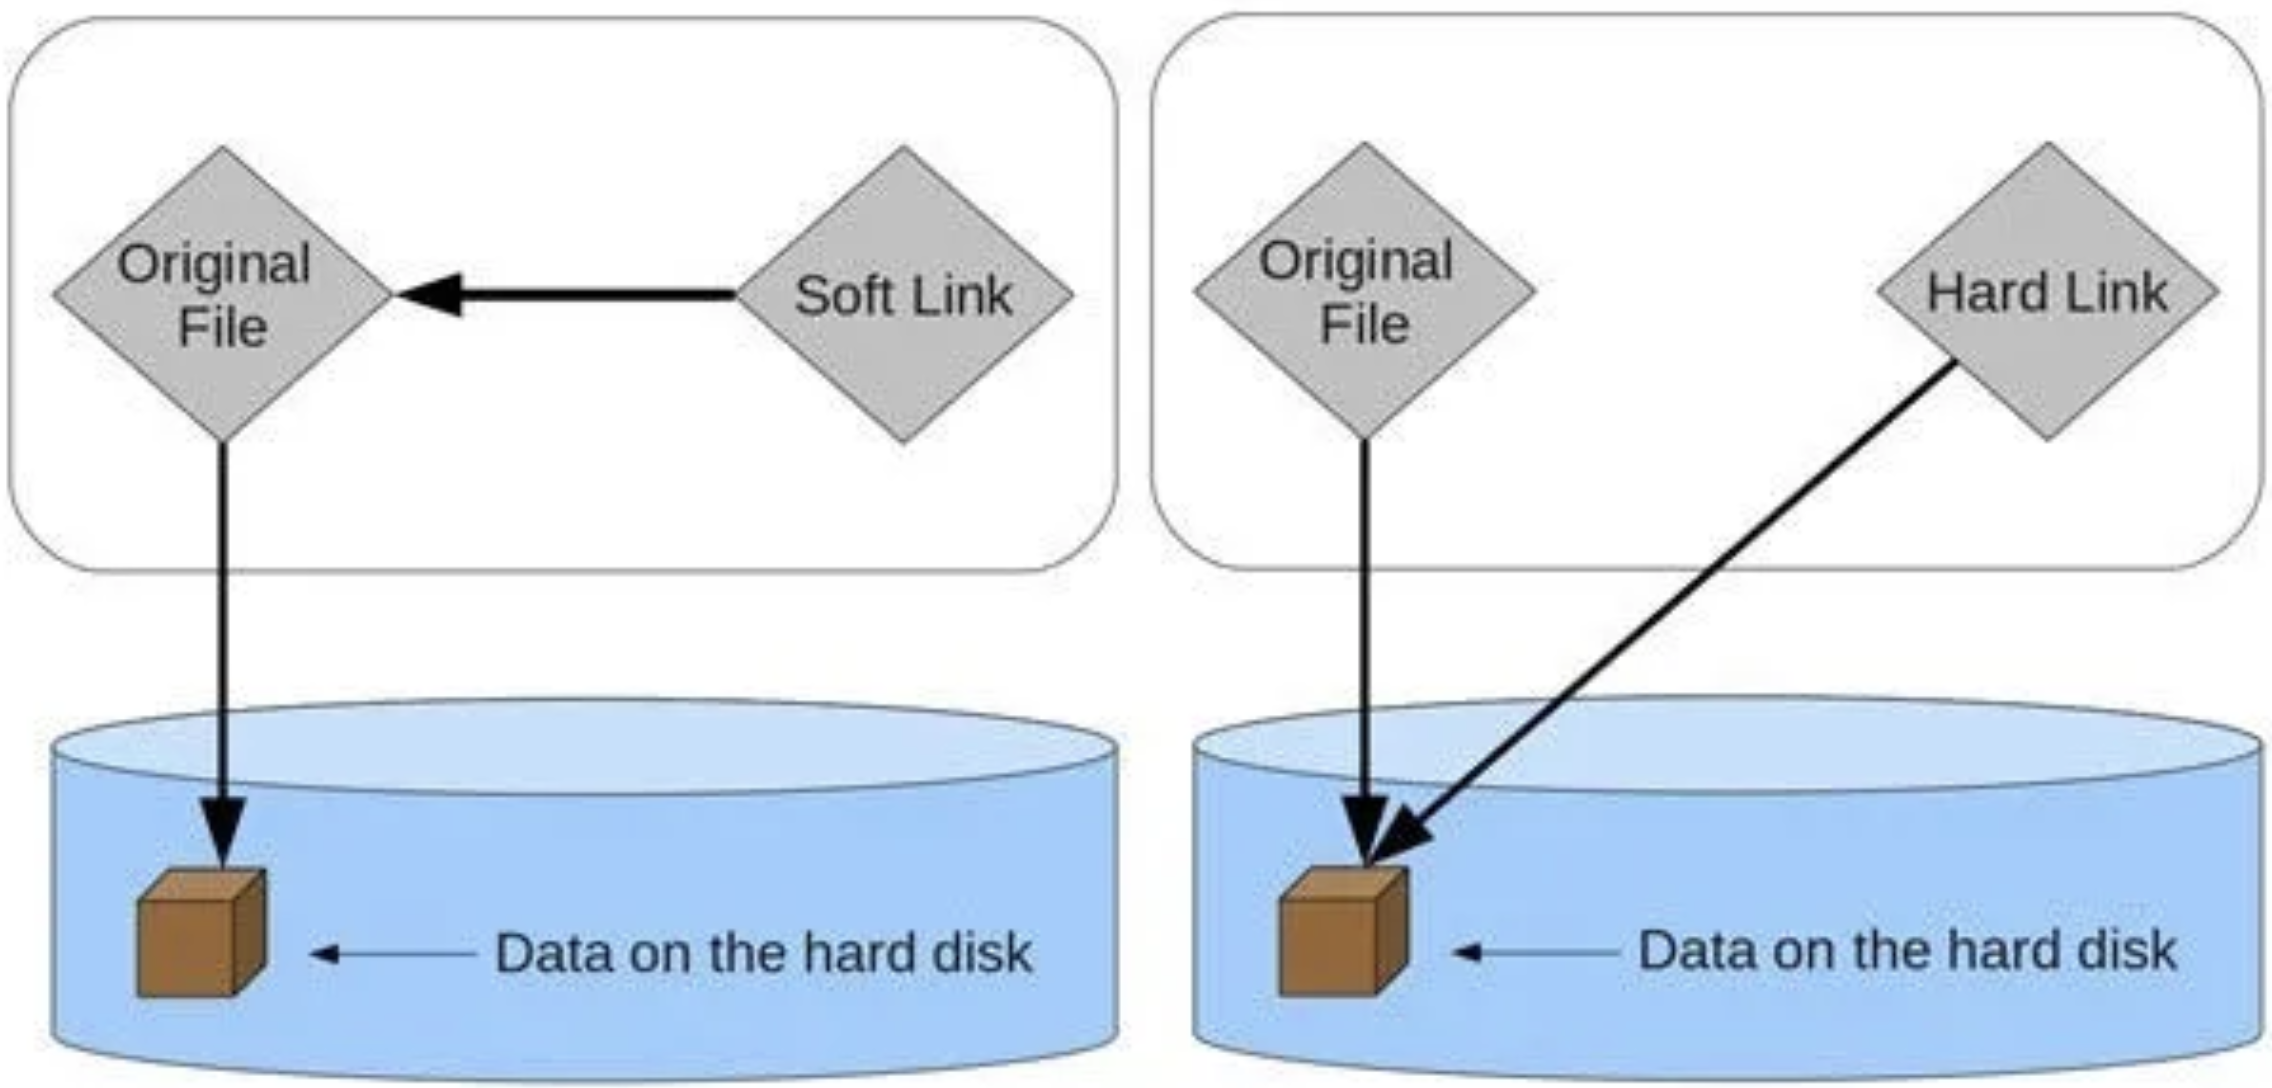
\includegraphics[width=0.93\textwidth]{images/soft-hard.png}
    \end{minipage}\\
- \textbf{Symbolic Link:} Logically maps a file's path to a target file by creating an actual link to the original file with a \textbf{new inode number}, and becomes broken or invalid if the target file is removed or deleted.\\
\noindent\textbf{File Allocation.} \\
Strategy to map file data to disk blocks. Managed via pointers in inodes or allocation tables.\\[2px]
\begin{minipage}[htp]{0.49\textwidth}
\noindent\textbf{File Allocation Table.}\\
\textbf{Layout:} A table holds block chains for files\\
\textbf{How it works:}
\begin{enumerate}[noitemsep,nolistsep,topsep=0px,partopsep=0pt,parsep=0pt]
    \item Inode contains pointer to first metadata block.
    \item Each Metadata block contains pointer to next metadata block.
    \item Read the corresponding data block in FAT table and repeat until end-of-file marker is reached.
\end{enumerate}

\textbf{Pros:} No ext. fragmentation, avoids mixing data and metadata, only requires locating the first block.\\
\textbf{Cons:} Poor random access, limited metadata, FAT must remain in memory.
\end{minipage}
\hfill
\begin{minipage}[htp]{0.49\textwidth}
\noindent\textbf{Contiguous Allocation.}\\
\textbf{Pros:} fast access, simple offset computation\\
\textbf{Cons:} fragmentation, difficult resizing\\
\textbf{Layout:} A file is a sequence of consecutive blocks\\[5px]
\noindent\textbf{Linked Allocation.}\\
\textbf{Pros:} No fragmentation, simple - find the first block of a file. \\\textbf{Cons:} slow random access, pointer overhead, mix data/metadata in the same block \\
\textbf{Layout:} Inode contains pointer to first block, each block contains pointer to next
\end{minipage}\\[2px]
\textbf{Multi-Level Indexing.} \\
Each inode holds pointers to data blocks directly or indirectly.\\
\noindent\textbf{Pros:} No ext. fragmentation, no conflating between data/metadata, Scales to large files, efficient for small files (via direct blocks), flexible block usage\\
\noindent\textbf{Cons:} Indirection overhead for large files, slower access for deep pointer chains.
\noindent\textbf{Inode Block Structure.} \\
Inode forms a fixed, asymmetric tree. Leaf nodes = fixed-size data blocks.
\begin{itemize}[noitemsep,topsep=0pt]
    \item \textbf{Pointers 0–11:} direct — point to data blocks
    \item \textbf{Pointer 12:} single indirect — points to block of data block pointers
    \item \textbf{Pointer 13:} double indirect — points to block of single indirect blocks
    \item \textbf{Pointer 14:} triple indirect — points to block of double indirect blocks
\end{itemize}
\vspace*{-10px}
\begin{center}
    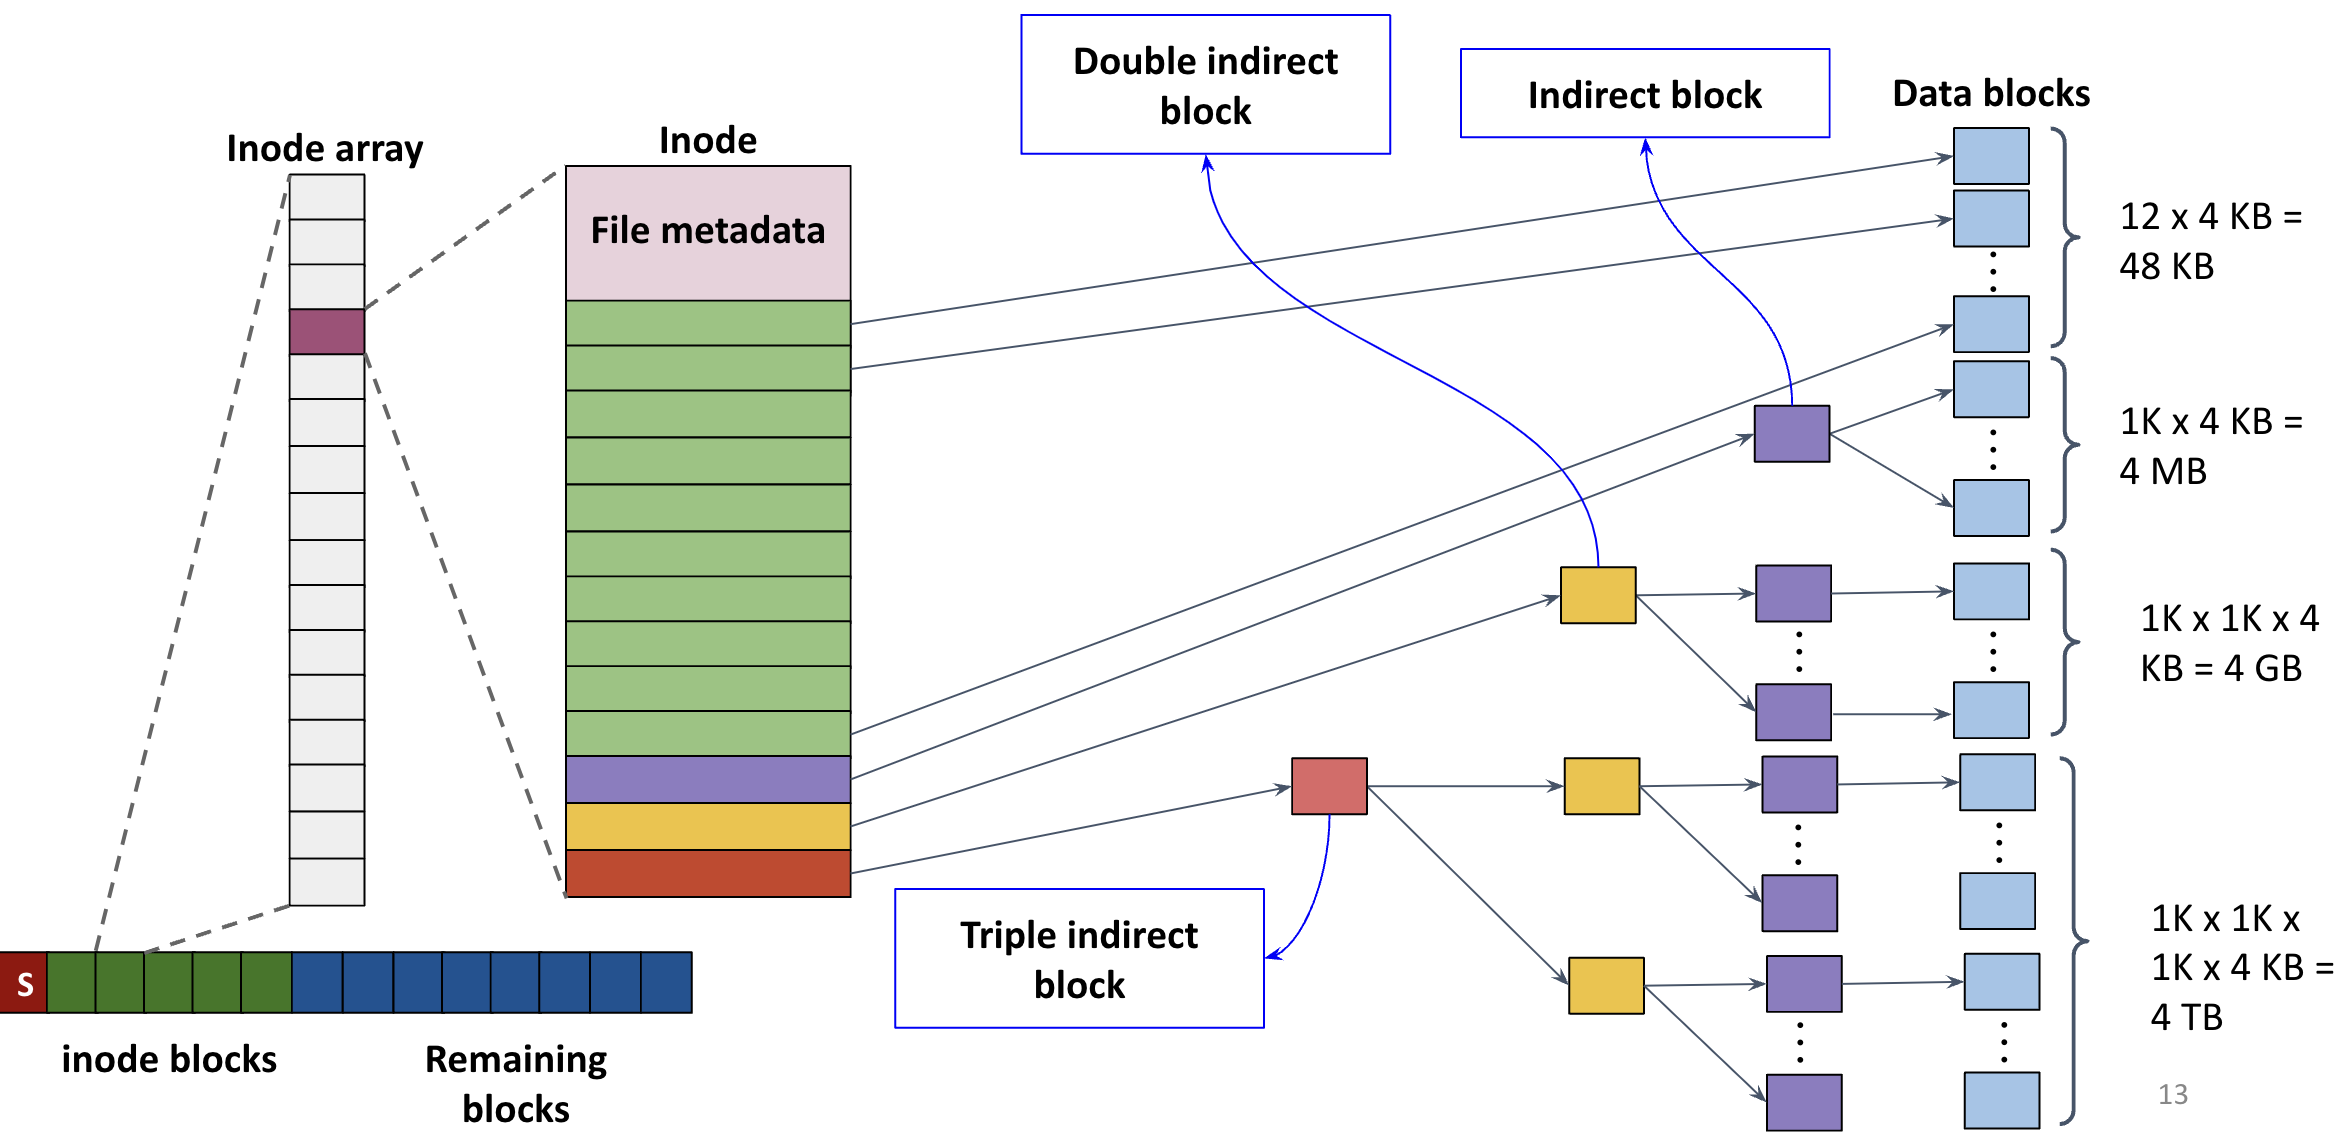
\includegraphics[width=0.95\textwidth]{images/multi-level-indexing.png}
\end{center}
\vspace*{-10px}
\begin{minipage}[htp]{0.4\textwidth}
    \small
\begin{itemize}[noitemsep,nolistsep,topsep=0px,partopsep=0pt,parsep=0pt]
    \item[] \textbf{Direct Pointers:} \\ 
$
    \texttt{number\_of\_direct\_pointers}
$
    
    \item[] \textbf{Single Indirect Pointer:} \\ 
$
    N = \frac{\texttt{block\_size} - r}{\texttt{pointer\_size}}
$
    
    \item[] \textbf{Double Indirect Pointer:} \\ 
$
    N^2 = \left(\frac{\texttt{block\_size} - r}{\texttt{pointer\_size}}\right)^2
$
\item[] \textbf{Triple Indirect Pointer:}  \\
$
    N^3 = \left(\frac{\texttt{block\_size} - r}{\texttt{pointer\_size}}\right)^3
$
\end{itemize}
\end{minipage}
\hspace*{-20px}
\begin{minipage}[htp]{0.68\textwidth}
    \small
\begin{itemize}[noitemsep,nolistsep,topsep=0px,partopsep=0pt,parsep=0pt]

    
    \item[] \textbf{Total Addressable Blocks:} \\ 
    \small
    $
    \texttt{number\_of\_direct\_pointers} + \sum_{i=1}^{3} \left(\frac{\texttt{block\_size} - r}{\texttt{pointer\_size}}\right)^i
$

    
    \item[] \textbf{Maximum File Size (bytes):} \\ 
$
    \texttt{total\_addressable\_blocks} \times \texttt{block\_size}
$
    \item[-] The count \(N\) represents the number of data blocks that can be reached through that single pointer.
    \item[-] If no metadata is reserved in the indirect blocks, then set \(r = 0\).
\end{itemize}
\end{minipage}
\begin{minipage}[htp]{1\textwidth}
    \noindent\textbf{Reading.}\\
    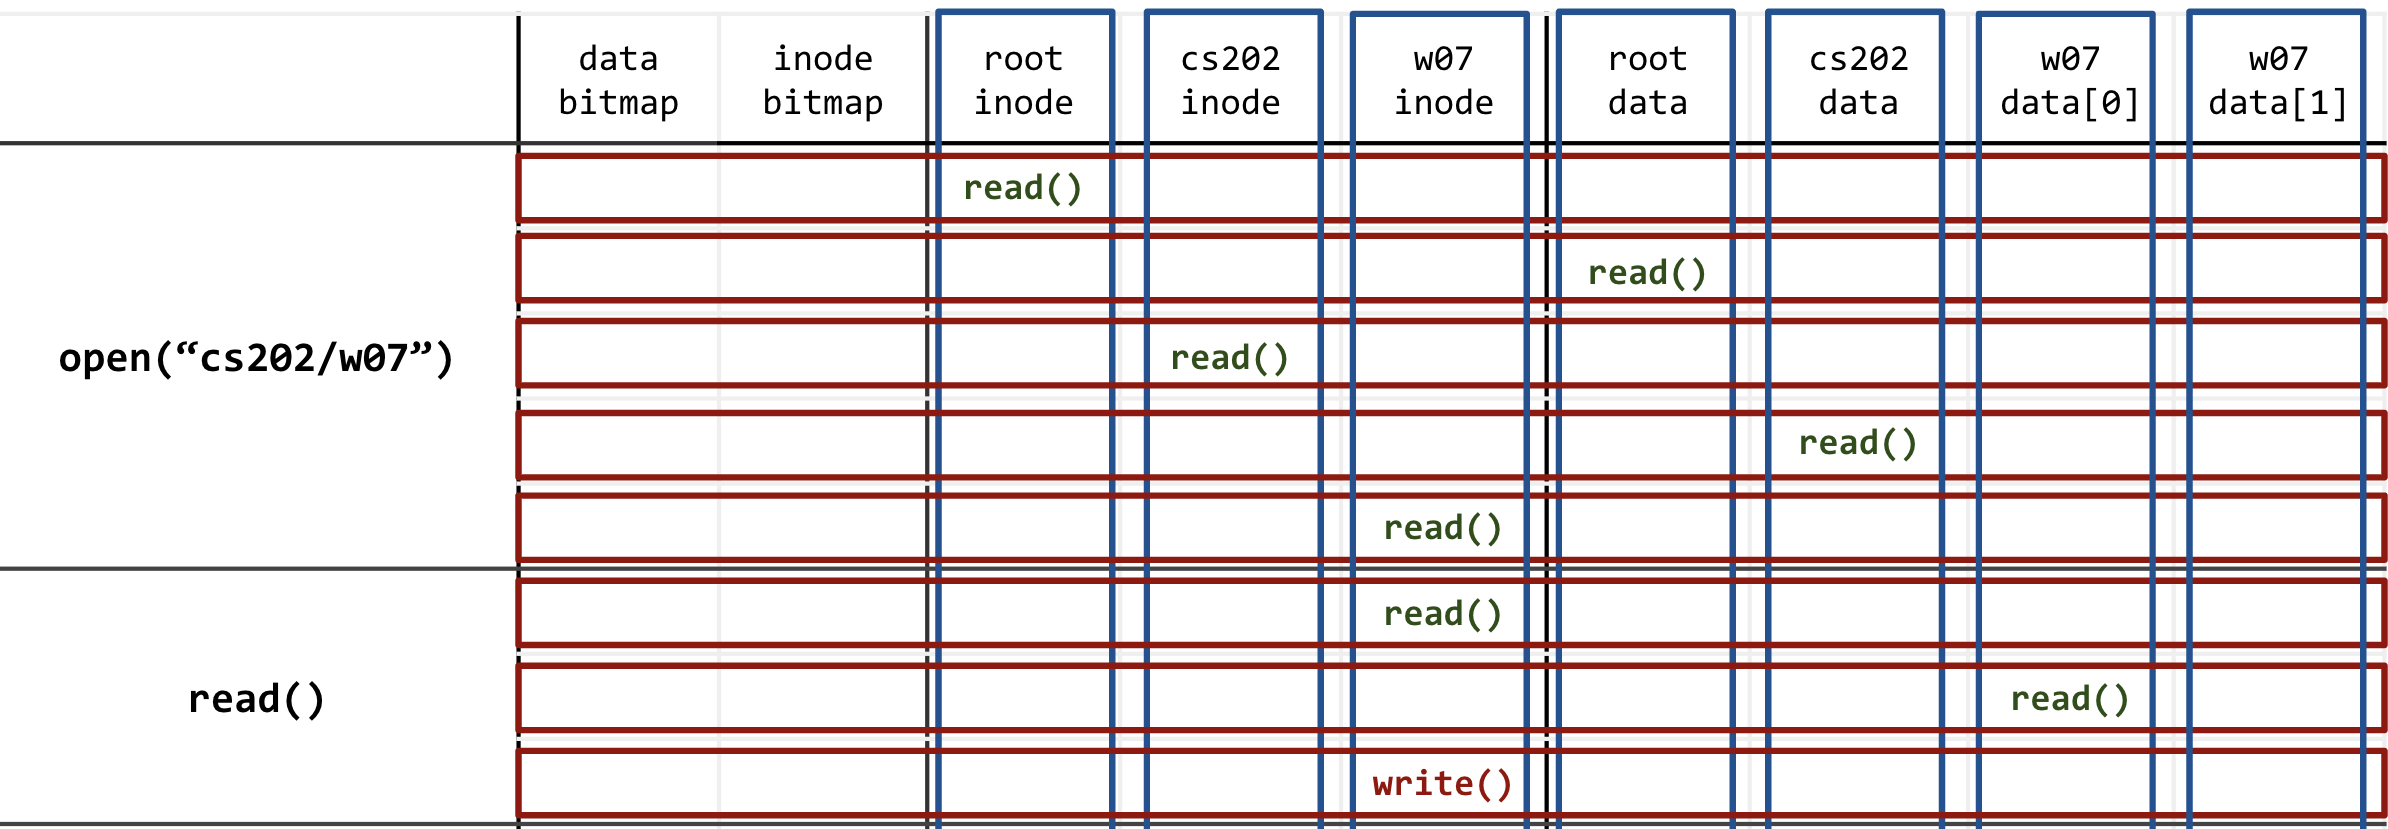
\includegraphics[width=1\textwidth]{images/read.png}
\end{minipage}\\
\begin{minipage}[htp]{1\textwidth}
    \noindent\textbf{Writing.}\\
    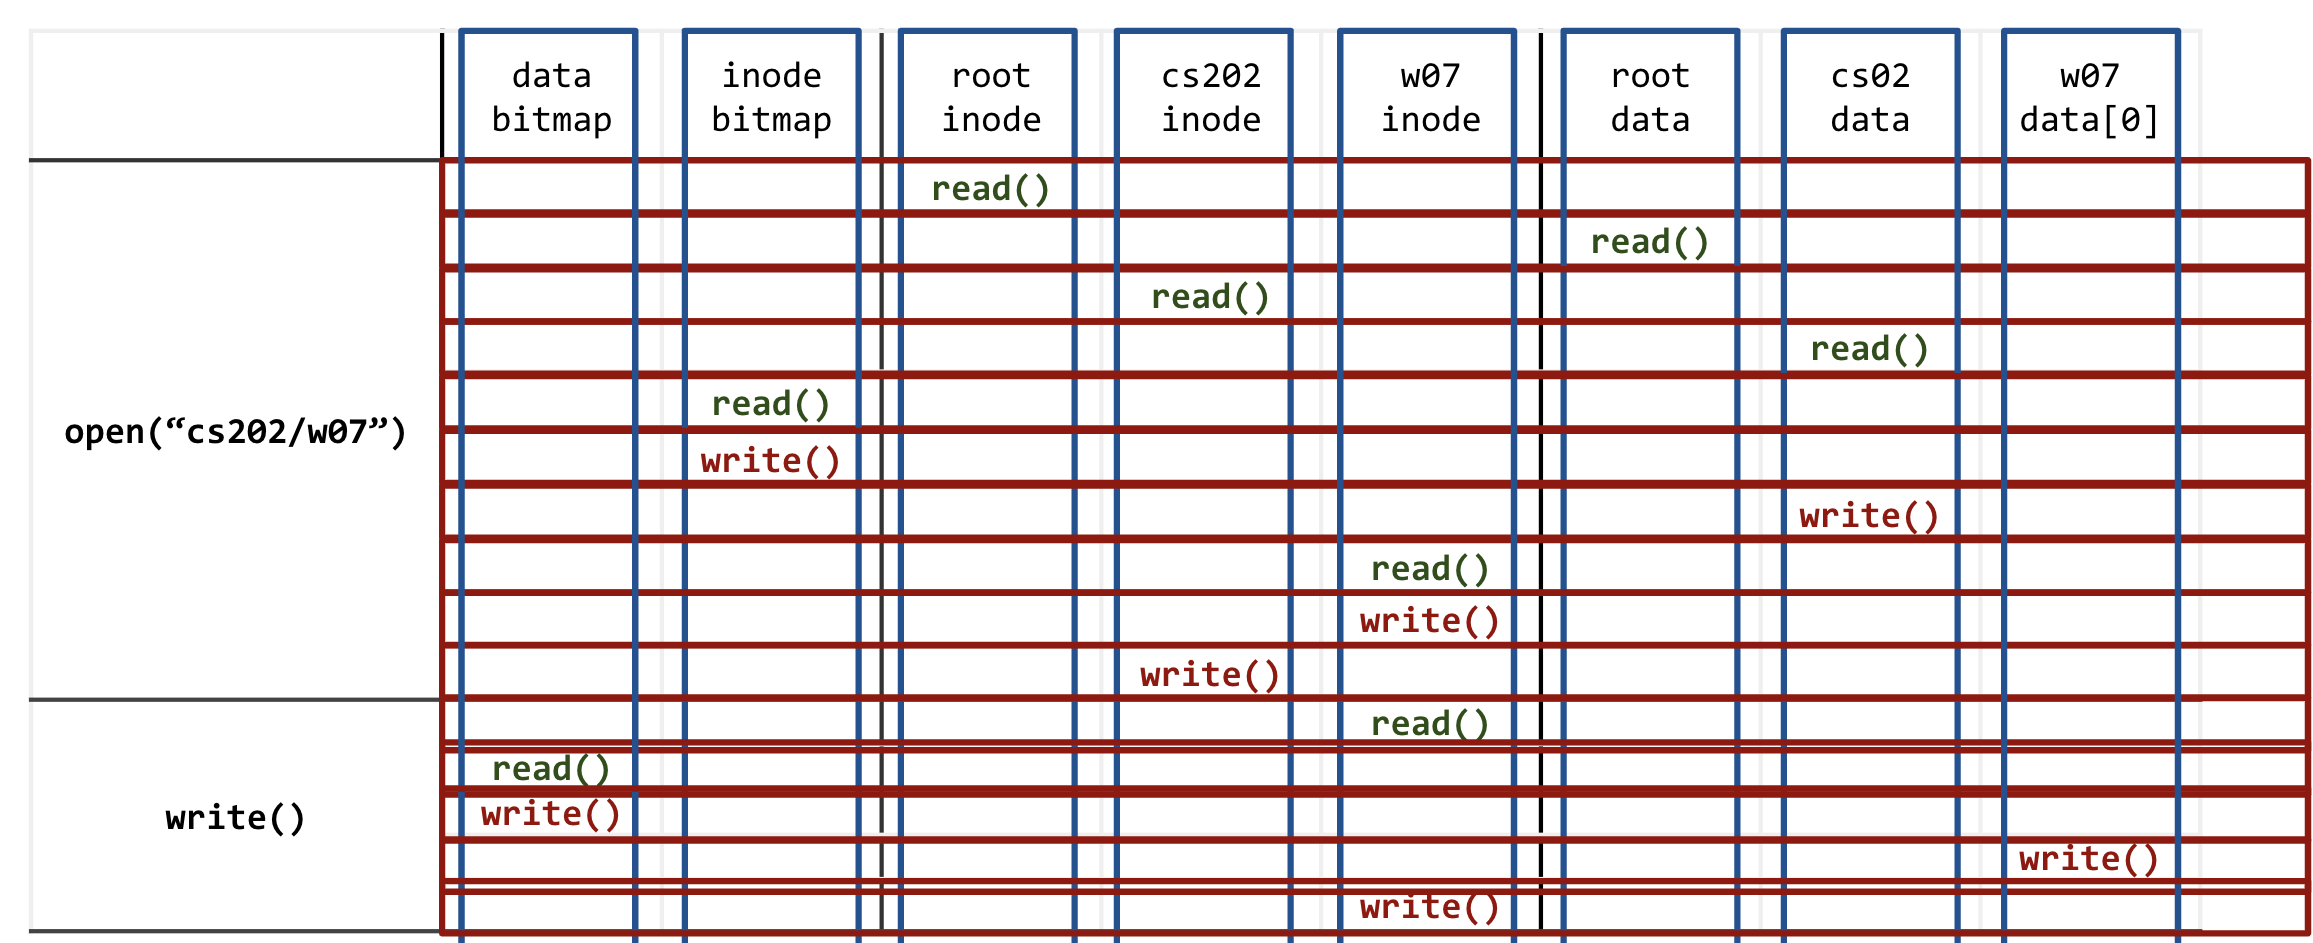
\includegraphics[width=1\textwidth]{images/write.png}
\end{minipage}
\end{minipage}
\newpage
\noindent
\hspace{-5px}
\begin{minipage}[t]{0.5\textwidth}
\begin{minipage}[t]{0.48\textwidth}
\noindent\textbf{Performance Metrics.}\\
- \textbf{Latency} — time per I/O ($\mu s$–$ms$)\\
- \textbf{Throughput} — data/sec ($MB/s$)\\
- \textbf{IOPS} — ops/sec\\
\noindent\textbf{Caching.} \\
Keep frequently accessed data in memory to reduce latency. Speeds up reads.\\
\noindent\textbf{Batching.} \\
Group multiple I/O operations to reduce syscall overhead and disk seeks.\\
\noindent\textbf{Block Cache.}\\
- In-memory cache of disk blocks\\
- \textbf{Good for reads} — avoids repeated disk access\\
\end{minipage}
\hfill
\begin{minipage}[t]{0.48\textwidth}\vspace{5px}
- \textbf{Limited for writes} — consistency requires flushing\\
\noindent\textbf{Write Caching.}\\
- \textbf{Write-through} — data written to both cache and disk immediately\\
  (slower, but consistent)\\
- \textbf{Write-back} — data stays in cache, flushed later\\
  (faster, but risk of data loss on crash)\\
- \texttt{fsync()} — forces flush of dirty blocks to disk\\
\end{minipage}\\[-7px]\hrule\vspace{3px}
\noindent\textbf{Consistency Update Problem.} \\
File system metadata may become inconsistent due to crashes during updates.\\
\noindent\textbf{File System Checker (fsck).} \\
Tool to scan and repair on-disk metadata inconsistencies.\\
Cons: Functionality - fix not always obvious or correct, \\Performance - slow; may take hours.\\
\noindent\textbf{fsck Fix Examples.}
\begin{itemize}[noitemsep,topsep=0pt]
    \item[-] \textbf{Link Count Inconsistency} — problem: inode's link count $\neq$ number of directory entries pointing to it; fix: correct link count to match actual references.
    
    \item[-] \textbf{Lost Inodes} — problem: inode has link count $ > 0$ but no directory entry points to it; fix: move file to \texttt{lost+found} for recovery.
    
    \item[-] \textbf{Data Bitmap Errors} — problem: inode uses a block, but bitmap marks it free; fix: set corresponding bitmap bit to “used”.
    
    \item[-] \textbf{Duplicate Pointers} — problem: two inodes point to same data block; fix: duplicate the block and update one inode to preserve both files.
    
    \item[-] \textbf{Invalid Pointers} — problem: inode points to a block beyond partition size; fix: remove invalid pointer to prevent access.
\end{itemize}
\noindent\textbf{Journaling.} \\
Crash-consistency technique. Metadata updates are first written to a log (journal) before applying to the main file system\\
\noindent\textbf{Pros.} Fast crash recovery (no full scan); Metadata consistency guaranteed; Safer than fsck in most cases.\\
\begin{minipage}[t]{0.48\textwidth}
\noindent\textbf{How It Works.}
\begin{enumerate}[noitemsep,topsep=0pt]
    \item Group changes into a \textbf{transaction}
    \item Write to journal: \texttt{TxBegin | changes | TxEnd | Valid}
    \item \texttt{Valid} block = transaction committed
    \item Apply changes to file system (checkpoint)
    \item Clear transaction from journal
\end{enumerate}
\end{minipage}
\hfill
\begin{minipage}[t]{0.48\textwidth}
\noindent\textbf{Recovery.}
\begin{enumerate}[noitemsep,topsep=0pt]
    \item For each uncleared transaction (stil in journal): 
    \item \textbf{If no \texttt{Valid}:} discard
    \item \textbf{If \texttt{Valid} found:} replay transaction to disk
\end{enumerate}
\end{minipage}\\[3px]
\hrule
\vspace{3px}
\begin{minipage}[t]{0.48\textwidth}
\noindent\textbf{I/O Interrupt.} \\
Device triggers an interrupt when it needs service. \\ 
\textbf{Pro:} efficient for unpredictable events.  \\
\textbf{Con:} high overhead per interrupt.\\
\vspace{-7.3px}
\hrule
\end{minipage}
\hfill
\begin{minipage}[t]{0.48\textwidth}
\noindent\textbf{I/O Polling.} \\
CPU repeatedly checks device status register.  \\
\textbf{Pro:} low overhead when frequent.  \\
\textbf{Con:} wastes CPU cycles if idle or infrequent.\\[2px]
\end{minipage}\\[-13px]
\noindent\textbf{Livelock.} \\
System busy handling I/O (e.g., interrupts) but makes no progress in real work. Spinning without forward progress.\\
\noindent\textbf{Real-World Strategy.}
\begin{itemize}[noitemsep,topsep=0pt]
    \item[-] Use \textbf{interrupts} for overlap (slow devices)
    \item[-] Use \textbf{polling} for short bursts, small data, high performance
    \item[-] \textbf{Coalescing}: delay, batch multiple responses for efficiency
\end{itemize}
\noindent\textbf{PIO (Programmed I/O).} \\
CPU tells the device \textbf{what data to read/write}.\\
\noindent\textbf{DMA (Direct Memory Access).} \\
CPU tells the device \textbf{where data is}.\\
\noindent\textbf{DMA Controller.} \\
Hardware unit that transfers data between device and memory without CPU involvement. Handles address incrementing and byte counting.\\
\begin{minipage}[htp]{0.48\textwidth}
\noindent\textbf{DMA Transfer Workflow. (device to memory transfer.)}
\begin{enumerate}[noitemsep,topsep=0pt]
\item The device driver receives an instruc-
    tion to transfer disk data to a buffer at
    address X.
\item The driver commands the disk con-
    troller to transfer C bytes from disk to
    the buffer at address X.
\item The disk controller initiates the DMA
    transfer operation.
\item The disk controller sends each byte to
    the DMA controller.
\item The DMA controller transfers bytes
    to buffer X, incrementing the memory
    address and decrementing C until C =
    0.
\item When C = 0, the DMA controller inter-
    rupts the CPU to signal completion of
    the transfer.
\end{enumerate}
\end{minipage}
\hfill
\begin{minipage}[htp]{0.48\textwidth}
\begin{center}
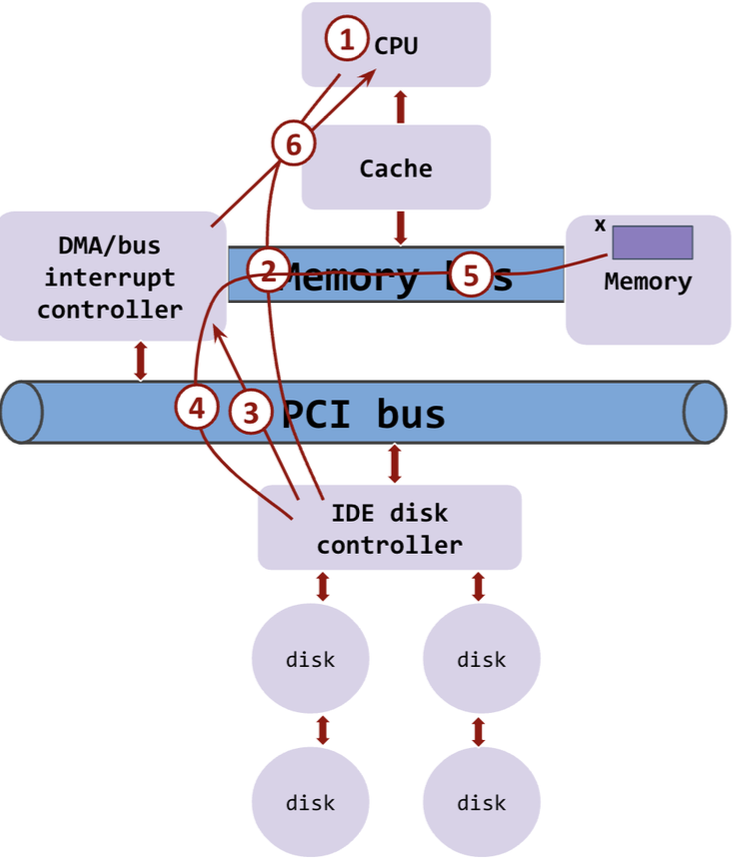
\includegraphics[width=0.85\textwidth]{images/dma.png}
\end{center}
\end{minipage}
\end{minipage}
\begin{minipage}[t]{0.5\textwidth}
    \noindent\textbf{Disk Storage} \\
    Goal: fast, reliable, affordable persistent data access. Must return what was written—quickly and without loss.\\
    \noindent\textbf{RAID (Redundant Array of Inexpensive Disks)} \\
    Combines multiple physical disks into one logical unit for performance and fault tolerance:\\
    Allows for a higher throughput and reliability.\\
     \begin{minipage}[htp]{0.48\textwidth}
            \textbf{RAID 0 (Striping)}\\
            data split across $N \geq 2$ disks\\
            \textbf{+} High throughput, full capacity\\
            \textbf{--} No redundancy\\
            \textbf{Read:} from corresponding disk\\
            \textbf{1 disk fails:} all data lost
        \end{minipage}
        \hfill
        \begin{minipage}[htp]{0.48\textwidth}
            \textbf{RAID 1 (Mirroring)}\\
            data duplicated on 2 disks\\
            \textbf{+} Survives 1-disk failure, fast reads\\
            \textbf{--} $2\times$ storage cost\\
            \textbf{Read:} from either copy (load-balanced)\\
            \textbf{1 disk fails:} use remaining mirror
        \end{minipage}\\
\begin{minipage}[htp]{0.48\textwidth}
            \textbf{RAID 5 (Striping + Parity)} — block-level striping + distributed parity across $N \geq 3$ disks\\
            \textbf{+} Efficient redundancy, survives 1-disk failure\\
            \textbf{--} Writes = read + modify parity (slow)\\
            \textbf{Read:} from data disk if intact\\
            \textbf{1 disk fails:} reconstruct via XOR:\\
$
                \text{Missing Block} = \text{Parity} \oplus \bigoplus_{i \neq \text{failed}} \text{Data}_i
$
            \\Or define parity as:\\
$
                \text{Parity} = \bigoplus_{i=1}^{N-1} \text{Data}_i
$
        \end{minipage}
        \hfill
        \begin{minipage}[htp]{0.48\textwidth}
            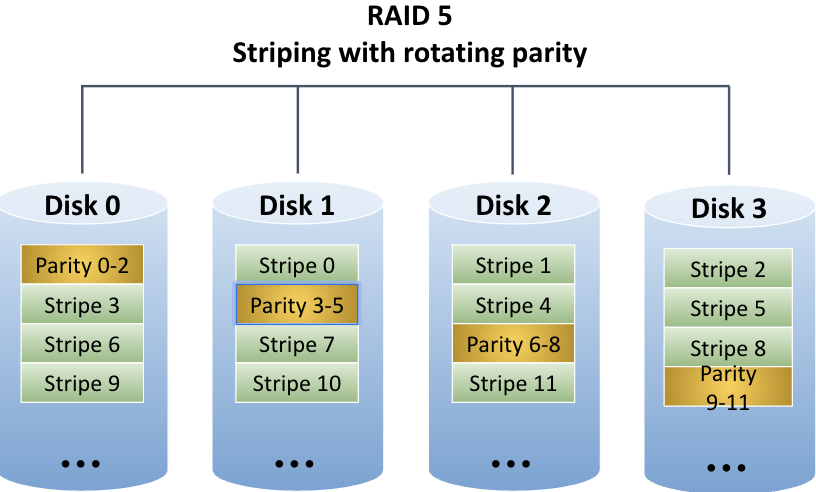
\includegraphics[width=1\textwidth]{images/raid5.png}
        \end{minipage}\\[3px]
        \hrule
        \vspace{3px}
        \noindent\textbf{Context Switch} \\
        Triggered by \textit{timer interrupt} or blocking events. Used to enforce fairness and preempt misbehaving threads.\\
        \textbf{Procedure.}
        \begin{enumerate}[noitemsep,topsep=0pt]
            \item \textbf{Save state} of current thread (PC, registers, etc.) to PCB
            \item \textbf{Choose next thread} via scheduler
            \item \textbf{Restore state} of selected thread from its PCB
            \item \textbf{Resume execution} via \texttt{return-from-trap}
        \end{enumerate}
        \noindent\textit{Timer interrupts} ensure control returns to the OS periodically, allowing preemption and preventing CPU hogging.\\
        \noindent\textbf{Scheduling Policy} — strategy for choosing the next thread
        
        \noindent\textbf{Scheduling Metrics}
        \begin{itemize}[noitemsep,topsep=0pt]
            \item[–] \textbf{CPU Utilization:} \% time CPU is busy
            \item[–] \textbf{Turnaround Time:} completion time $-$ submission time
            \item[–] \textbf{Response Time:} time from submission to first response (eg. submission to first time a thread is scheduled)
        \end{itemize}
        \begin{minipage}[t]{0.48\textwidth}
        \noindent\textbf{FIFO Scheduling (First-In, First-Out)} \\
        Non-preemptive (waits for completion before scheduling next thread). Runs threads in order of arrival.

        \begin{enumerate}[noitemsep,topsep=0pt]
            \item \textbf{Enqueue} new threads at the tail of the ready queue
            \item \textbf{Select} the thread at the head of the queue
            \item \textbf{Run} it to completion or blocking
            \item \textbf{Repeat} with the next thread in queue
        \end{enumerate}
        \noindent\textbf{Pros:} Simple, fair (by arrival order), minimal overhead \\
        \noindent\textbf{Cons:} Poor responsiveness, suffers from \textit{convoy effect} (short jobs wait behind long ones)\\
        \end{minipage}
        \hfill
        \begin{minipage}[t]{0.48\textwidth}
        \noindent\textbf{SJF Scheduling (Shortest Job First)} \\
        Non-preemptive. Picks the thread with the shortest remaining execution time.
        \begin{enumerate}[noitemsep,topsep=0pt]
            \item \textbf{Estimate} or know job lengths in advance
            \item \textbf{Select} the shortest job from the ready queue
            \item \textbf{Run} it to completion or blocking
            \item \textbf{Repeat} with the next shortest job
        \end{enumerate}
        \vspace{4px}
        \noindent\textbf{Pros} Minimizes average turnaround time (optimal under perfect knowledge) \\
        \noindent\textbf{Cons} Requires job length estimates, risk of starvation for long jobs\\
        \end{minipage}\\
        \noindent\textbf{STCF Scheduling (Shortest Time to Completion First)} \\
        Preemptive SJF. Always runs the thread with the least remaining time.
        \begin{enumerate}[noitemsep,topsep=0pt]
            \item \textbf{Track} remaining time for all ready/running threads
            \item \textbf{On arrival} of a new thread, compare its time to current thread
            \item \textbf{Preempt} if new thread has shorter remaining time
            \item \textbf{Run} the shortest job until completion or preemption
        \end{enumerate}

        \noindent\textbf{Pros} Optimal average turnaround time under preemption \\
        \noindent\textbf{Cons} Requires accurate time estimates, may cause starvation of longer jobs, bad Response Time\\
        \noindent\textbf{Round Robin Scheduling} \\
        Preemptive. Each thread gets a fixed time slice, cycling through the ready queue.\\
        \begin{minipage}[htp]{0.48\textwidth}
        \begin{enumerate}[noitemsep,topsep=0pt]
            \item \textbf{Enqueue} threads in arrival order
            \item \textbf{Run} the thread at the head for one quantum
            \item \textbf{Preempt} if not finished; move to tail of queue
            \item \textbf{Repeat} with the next thread in queue
        \end{enumerate}
        \end{minipage}
        \hfill
        \begin{minipage}[htp]{0.48\textwidth}
            \begin{center}
                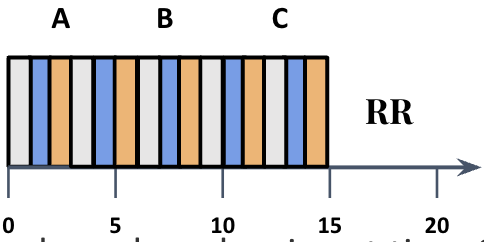
\includegraphics[width=0.8\textwidth]{images/round-robin.png}
            \end{center}
        \end{minipage}\\
        \noindent\textbf{Pros} Fair, responsive, avoids starvation \\
        \noindent\textbf{Cons} High context switch overhead if time slice is too small; poor for short jobs if time slice is too large\\
        \noindent\textbf{MLFQ Scheduling (Multi-Level Feedback Queue)} \\
        Preemptive. Dynamically adjusts thread priority based on behavior.\\
        \noindent\textbf{Rules}
        \begin{enumerate}[noitemsep,topsep=0pt]
            \item If priority(A) $>$ priority(B), \textbf{A runs}
            \item If priority(A) = priority(B), \textbf{A, B run in Round Robin}
            \item \textbf{New threads start at top priority}
            \item If a thread uses up its time slice, \textbf{demote its priority}
            \item Periodically \textbf{boost all threads to top priority} (prevents starvation)
        \end{enumerate}
        \begin{minipage}[htp]{0.48\textwidth}
        \noindent\textbf{Procedure}
        \begin{enumerate}[noitemsep,topsep=0pt]
            \item Maintain multiple ready queues by priority level
            \item Insert new or boosted threads at highest priority
            \item Select thread from highest non-empty queue
            \item Run using Round Robin within queue
            \item \textbf{Demote if thread uses full time slice; \textbf{boost} periodically} !!!!
        \end{enumerate}
        \end{minipage}
        \hfill
        \begin{minipage}[htp]{0.48\textwidth}
        \begin{center}
            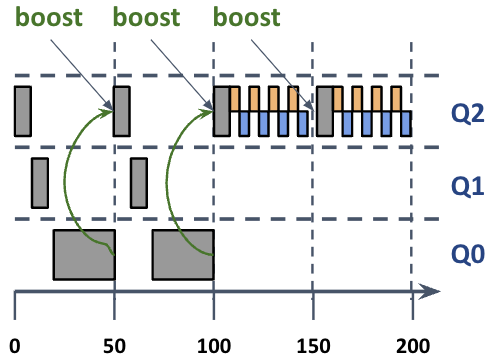
\includegraphics[width=0.8\textwidth]{images/mlfq.png}
        \end{center}
        \end{minipage}
    \end{minipage}
    
\end{document}